\documentclass[paper=a4, fontsize=11pt, twoside, BCOR=12mm, parskip=full, listof=totoc]{scrreprt}
\linespread{1}
% Some general settings
\KOMAoptions{headsepline=true, abstract=true, bibliography=totoc, DIV=12}
% Some useful packages
\usepackage[utf8]{inputenc}		% character encoding
%\usepackage[T1]{fontenc}
\usepackage[english]{babel}		% English language	
\usepackage{amsmath, amsthm, amssymb}	% Math environments for equations and some more stuff
\usepackage{tocloft}
\usepackage{amsfonts}
\usepackage{graphicx, tikz}		% Graphics and drawing with tikz
\usetikzlibrary{positioning, arrows}
\usepackage{pgfplots}
\pgfplotsset{compat=1.17, width=11cm}
\usepackage{eurosym}			% Euro-symbol
\usepackage[hidelinks]{hyperref}	% Hyperlinks
\usepackage{subcaption} % for placing multiple images at a certain locatin next to each other
\usepackage{empheq}  
%\usepackage[numbers,sort&compress,square]{natbib} %%bibstyle
\usepackage{bbm}
\usepackage{float}
\usepackage{booktabs}
\DeclareOldFontCommand{\bf}{\normalfont\bfseries}{\mathbf}
%
% this ensures we have numbered paragraphs
%
\setcounter{secnumdepth}{4}
% Some theorem styles, numbering starts new with each chapter
%\theoremstyle{plain}
%   \newtheorem{lem}{Lemma}[chapter]
%   \newtheorem{thm}{Theorem}[chapter]
%   \newtheorem{prop}{Proposition}[chapter]
%   \newtheorem{coro}{Corollary}[chapter]

%\theoremstyle{definition}
%   \newtheorem{ex}{Example}[chapter]
%   \newtheorem{defi}{Definition}[chapter]

%\theoremstyle{remark}
%   \newtheorem{rem}{Remark}[chapter]
% Some Layout things
\pagestyle{headings}	% Headings on each page
\setkomafont{author}{\usekomafont{subtitle}}	% Fonts on the titlepage
\setkomafont{date}{\usekomafont{subtitle}}
\setkomafont{subject}{\usekomafont{subtitle}}
\setkomafont{publishers}{\usekomafont{subtitle}\large\mdseries}
\addtokomafont{dedication}{\normalsize}

% Put the uni-logo at the top right of the titlepage and add line with the study program
\subject{\hspace*{\fill}
\includegraphics[width=5cm]{uniFB3-logo.pdf}}
\subtitle{\vspace*{1cm}Master Thesis\\Mathematical Modeling Of Complex Systems\vspace*{1cm}}


% Title of the thesis
% Author name and matriculation number
% Date of submission
% Names and Affiliation of the examiners
\title{Modeling infectious diseases in mixed household structures}
\newcommand{\myname}{Shrawan Parajuli}
\newcommand{\mystudno}{218101021}
\newcommand{\myplace}{Koblenz}
\newcommand{\submissiondate}{28.11.2023}

\publishers{\begin{tabular}{lp{6cm}}
	First Examiner: &Prof.Dr.~Thomas Götz\newline Mathematical Institute\newline University of Koblenz\\[1ex]
	Second Examiner: &Dr.~Radomir Pestow\newline Mathematical Institute\newline University of Koblenz
	\end{tabular}}

% No need to change this
\author{\myname\\Matr.No.~\mystudno}
\date{\myplace, \submissiondate}

% If you want to thank some one - here's the place to do so.
%\dedication{\flushleft This thesis is dedicated to Prof.Dr.~Thomas Götz for drawing my attention to this fascinating problem.}

%
% Here begins the main part
%
\begin{document}
\maketitle
\pagenumbering{roman}
 
% That's more-or-less the standard text for the declaration of authorship.
\addchap*{Declaration of authorship}
I herewith confirm that I alone have authored this thesis, that I did not use any resources other than those I have cited - in particular, no online sources not listed in the bibliography section - and that I have not previously submitted this thesis in association with any other examination procedure.\\

\vspace*{2cm}
\rule{3.5cm}{.5pt}\\
\myname\\
\myplace, \submissiondate

\addchap*{Abstract}
We studied SIS model of infectious disease in single household of size two. For 		this we introduced master equation and studied the transition of household state  with focus on the influence of infection and recovery parameters. We performed a simulation using Runge-Kutta method to observe the influence of these parameters. The steady state observed in the simulation was further investigated by Linearization around equlibrium points which showed the existence of disease-free equilibrium and endemic equilibrium. Notably, our observations indicated that an increase in infection parameters lead to endemic equilibrium and an increase in recovery parameter leads disease-free equilibrium. 
\addchap*{Acknowledgment}
I would like to express my sincere gratitude to Prof.Dr.Thomas Götz for his guidance throughout this work. His formative feedback, patience and motivation helped me to complete my Master’s thesis. 
My special thanks to Dr. Christian Kahle for making the Latex template available which simplified the process of preparing the report.
I would like to thank my family and friends who constantly guided and supported me.
\newpage
%\cleardoublepage
\pagenumbering{arabic}
\tableofcontents
\newpage
%\cleardoublepage
\listoftables
\cleardoublepage
\listoffigures

%
\setlength{\parindent}{0pt}

\newtheorem{definition}{Definition}[section]

%
% Macro for the formulation of external infection rate epsilon in SHH case
% must be used in a Math environment
\newcommand{\epsSHH}[0]{ ( \frac{\alpha}{\bf{N}} \sum_{k=1}^{\bf N}kP_k ) }
%
% Macro for the formulation of external infaction rate epsilon in the MSSHH case
%
%\newcommand{\epsiMSSHH}[0]{ ( \frac{\bf{M}}{\bf{P}} \sum_{k=1}^{S}  k \sum_{l=1}^{S} r_l p_{k,l})}
%
% Macro for the formulation of external infection rate epsilon in SHH case
% for N:=2
% must be used in a Math environment
\newcommand{\epsSHHTwo}[0]{(\frac{\alpha}{\bf{2}} P_1+{\alpha} P_2)}
%\newcommand{\epsSHHThree}[0]{(\frac{\alpha}{\bf{2}} P_1+{\alpha} P_2+{\alpha} P_3)}
%
% Makro for big fat "TODO"
\newcommand{\TODO}[1]{\par {\bf \large TODO:} {\texttt #1 }}
%mm
% macro for a remark from Jochen
\newcommand{\JL}[1]{\par {\bf \tiny remark (jl):} {\tiny \texttt #1 }}

% Makro for big fat "NOTE"
\newcommand{\Note}[1]{\par {\bf \large Note:} {\emph #1 }}

%
% Macro for indicator function ("i lower_equal k")
%
\newcommand{\charfleq}[1]{{X}_{\{\leq #1\}}}


%
% Macro for indicator function ("i greater_equal k")
%
\newcommand{\charfgeq}[1]{{X}_{ \{\geq #1 \}}}
%
% this ensures we have numbered paragraphs
%
\setcounter{secnumdepth}{4}

%%%
%%% Here starts the real work
\chapter{Introduction}
Throughout historical recorded event, the abrupt emergence of infectious diseases have been concerning for human population\cite{dadlani2020deterministic}. The regions where diseases occur might gradually decrease possibly due to immunity or development of vaccine but also might become endemic due to possible lack of health care facilities \cite{brauer2017mathematical}. Epidemiological studies deals with the occurrence of epidemic diseases, its spread and control\cite{dadlani2020deterministic}. And, the goal of epidemiologists is to take the intial step by collecting the data of disease movement, observing the key events, analyzing the cause and predicting with realistic approach should become the ultimate goal in controlling it \cite{brauer2017mathematical}.\\ 
  
Brauer \cite{brauer2017mathematical} credits public health physicians for using mathematical models such as compartmental models to understand the spread of infection. He also mention that the core idea of mathematical epidemiology of basic reproduction number was introduced by Dr.Ross for understanding dynamics of disease specially for malaria. Kermack and Mckendrick also formulated epidemic model where they established a threshold value for which an outbreak can be considered epidemic if it exceeded that value\cite{hethcote2000mathematics}.\\

Mathematical modeling has become an integral part of understanding mechanisms and behaviour in epidemiology. In other words, mathematical models are valuable tools for estimating strategies to understand the transmission of infectious diseases. It is a comprehensive abstraction represented by the formulation of equations to estimate an event. The model's premise about variables and parameters may help in estimating the epidemic. Mathematical modeling is a useful tool to simulate and analyze events which help us reach conclusion. \cite{hethcote2000mathematics}.\\

For applied mathematicians, the main question in disease models would be to solve solutions analytically and its qualitative behavior. And concerning question for mathematical epidemiologists would be about circumstances and persistence of a disease. Another concern for epidemic modelers would be investigation of models behavior at equilibrium on given initial conditions.\cite{sattenspiel1990modeling}. The analytical approach to equilibrium begins with finding constant solutions \cite{brauer2017mathematical}. Disease-free equilibrium and endemic equilibrium were studied in \cite{egbetade2018local} using SIR Model by local stability of the equilibrium points and the basic reproduction number. Dadlani \cite{dadlani2020deterministic} also investigated disease-free equilibrium and endemic equilibrium with different models, including the SIS model with linear stability and reproduction number.\\ 

It is often observed and compared that the transmission rate of an infection is higher within a household which affects a small number of individuals to outside household which affects higher number of individuals. Wide-ranging studies of infectious disease model has been based on household-structured model. This study of discrepencies in household-structured of population has helped in understanding the pattern of diseases transmission to advise possible control policies and intervention strategies like household-based vaccination strategies for influenza and treatment of infected individual and their contacts for yaws\cite{holmes2022approximating}. \\

A typical method for aligning a household model with data is to assume that the system is in a state of steady equilibrium. Followed by establishing a connection between the external force of infection and infections occurring in other households\cite{holmes2022approximating}. Limitations of household state in SIA model in finite number household size lead \cite{holmes2022approximating} to use SIS model in their studies with different numbers of household of same size using master equation. In thesis we also use master equation based on SIS model to analyze equilibria for household of size two.\\

The structure of this thesis unfolds in Chapter 2, where we present a section on the general derivation of master equation, its SIS dynamics within a single household approximation and analyzing solutions in terms of equilibrium. Chapter 3 delves into initial conditions through numerical simulations and analyze equilibria. In Chapter 4, we discuss the outcomes of Chapter 3 offering a comparative analysis of results and its limitations and suggestion for future research and Chapter 5 we concludes our thesis.

\chapter{Model and Method}
A model is a portray of events in simple structure to obtain the crucial fundamental characteristic factor of the system and to explain its noticeable phenomena. Based on biological nature of infection and demography in population there is transmission dynamic model and static model. Transmission dynamic model depends on prevalence of infection which changes with time as a function whereas static model is independent of time. In deterministic model, the average life of an infection whose course of infection is based on same predefined model of parameters and initial condtions while stochastic model is random processes. The state of disease with similar characteristic in an individual is considered in homogenous population and with different characteristic is consdidered in heterogenous popluation \cite{Mishraetal}.\\ 

Kessler \cite{kessler2008epidemic} compares two models susceptible-infected-susceptible (SIS) with susceptible-infected-recovered (SIR). In his comparision,reinfection to a recovered individual is allowed but in SIR model reinfection is not allowed. Similarity is shown in the case of SIS and SIR model when the infection level of diseases is below threshold value and infection dies out for both models. On the contrast outcome might be different for both model when infection level is above threshold value. While in the SIS model the number of susceptible individuals may increase, the number of susceptible individuals in the SIR model can only decrease.\\

 In this chapter we derive general master equation for a single household (SHH) with view of SIS Model. The transmission of an infectious disease is viewed from its phenomenological derivation with concept of SHH approximation in equation (4) of \cite{holmes2022approximating}. 
%SIS mode

\pagebreak
\section{ Derivation of Master Equations for the Single Household Model(SHH)}
In this section, we will apply idea of SIS model in single household structure with different sizes in population. An introduction to parameters influencing single household size SHH are given below with description. 

\begin{table}[H]
	\centering 
	\caption{Defination of parameters}
	\label{Defination of parameter}
	\begin{tabular}{cl}
	\toprule     
     Parameter & Description  \\
    \midrule
	  $\epsilon$  & External Infection Rate in which \emph{individual} gets infected from an external \\ & source outside household and brings infection inside household \\
	  $\bf{T_p}$   & Total individual in population \\
	  $\bf{N}$ &  Overall Number of Individuals in Household\\
      $\beta$ & The Internal Infection Rate in which an \emph{individual} gets infected from an \\ & internal source inside household \\
      $\gamma$  &  Recovery Rate in which a susceptible \emph{individual} recovers \\
	\bottomrule
	\end{tabular}
	
\end{table}

\subsection*{Dependence of External Infection Rate on the Probability Distribution}
It is plausible that the external infection rate $\epsilon$ is not constant, but rather depends on the rate of infected people in the population.
We may thus \emph{assume} that epsilon is a linear function of the infection rate $\frac{I}{T_p}$, say $\epsilon=\tilde{\alpha}\frac{I}{T_p}$ with a suitable proportional factor $\tilde{\alpha}$.
\\
However, in the SHH Model, in general we do not have the explicit number of infected people ($I$). Instead, we have expectation values for this number, so in what follows, we have to base the definition of external infection for our model on these expectation values.
\\
\\
Let $P_k$ denote the probability that in a given household we have k infected individals.
As the different households are indistinguishable, we can assume that the probability distribution $(P_0,P_1,...,P_N)$ is the same in each household, 
and based on this assumption of homogeneous distributions we may approximate the number of infected people in each individual household (say $\mathbb{E}I_H$) 
by its expectation: $\mathbb{E}I_H=\sum_{k=0}^N k*P_k$.
\\
\\
The expectation value for the number of infected individuals in a given household by definition is $\mathbb{E}I_H=\sum_{k=0}^Nk*P_k$.
\\
Denoting ad-hoc the number of households in the model with $M_H$, the expectation for the overall number of infected people in the population becomes $M_H*\mathbb{E}I_H$, 
while the overall number of people in the population $T_p$ can be written as $M_H*N$.
\\
Thus, we get an approximation $\frac{I}{T_p} \approx \frac{M_H*\mathbb{E}I_H}{M_H*N}=\frac{\mathbb{E}I_H}{N}=\frac{1}{N}{\sum_{k=0}^N kP_k}$
\\

\subsubsection*{Introducing the $\alpha$ Parameter}
These considerations lead to assuming that there is a proportional factor $\alpha$ linking the external infection rate $\epsilon$ 
to the expectation value of infected individuals in a household:

For the external infection rate $\epsilon$ In the SHH-N Model we have 
$$\epsilon=\frac{\alpha}{N}{\mathbb{E}I_H}=\frac{\alpha}{N}{\sum_{k=0}^N kP_k}$$
with a suitable parameter alpha.
\subsection*{Master Equations for the General SHH Case}
	We begin analyizing SIS dynamics in SHH with referring to set of master equations from equation (4) from \cite{holmes2022approximating}.  
	For a system that can take on a finite  number of states $S_0,..,S_N$, let $P_k$ and $P_l$ be the probabilities of the system in state $k$ and state $l$.
We then have the general form of the  Master equations\cite{masterequation}:

\begin{equation}
        \label{1stgeneral_discrete_master_equation1st}
\frac{dP_k}{dt} = \sum_{l \ne k} (T_{lk}P_l-T_{kl}P_k)  
\end{equation}

Where the $T_{lk}$ is the transition probabilty for a state change from $S_l$ to $S_k$ and $T_{kl}$ is the transition probabilty for a state change from $S_k$ to $S_l$.
In the case of a single household model where the state $S_k$ means we have exactly $k$ infected and $N-k$ susceptible individuals of the household, the master equations becomes more simple, as state transitions can appear from $S_k$ to $S_{k+1}$ or from $S_{k+1}$ to $S_{k}$ and also state transitions can appear from $S_k$ to $S_{k-1}$ or from $S_{k-1}$ to $S_{k}$.
%	
The general form of the  master equations can be written as:
\begin{equation}
	\label{general_discrete_master_equation} 
\frac{dP_k}{dt} =T_{(k-1)k}P_{k-1}-T_{k(k-1)}P_k+T_{(k+1)k}P_{k+1}-T_{k(k+1)}P_k 
\end{equation}  
\\	% could we write in matrix form 
	Where the $T_{(k-1)k}$, $T_{k(k-1)}$, $T_{(k+1)k}$, $T_{k(k+1)}$ are the transition probabilties for a state change from $S_{k-1}$ to $S_k$ or $S_k$ to $S_{k-1}$ and $S_{k+1}$ to $S_k$ or from $S_k$ to $S_{k+1}$. From here on, also the convention is taken that when dealing with households of size N, $P_k=0$ if $k<0$ and $N>k$ is adopted. For derivation of single household equation which we will use on indicator function\cite{indicatorfunction}.
	Below shows the diagram of state transition in SHH

\begin{figure}[H]
\centering
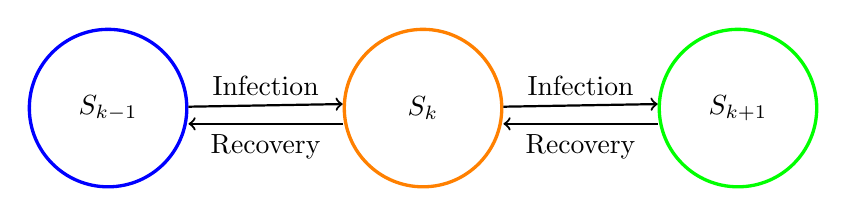
\begin{tikzpicture}[node distance=4cm, auto]
    % Define nodes
    \node [draw=orange, very thick, circle, minimum size=2cm] (Si) {$S_k$};
    \node [draw=blue, very thick, circle, minimum size=2cm, left of=Si] (Siminus) {$S_{k-1}$};
    \node [draw=green, very thick, circle, minimum size=2cm, right of=Si] (Siplus) {$S_{k+1}$};
    
    % Arrows from Sk-1 to Si and from Sk to Sk-1
    \draw[->, thick] ([yshift=0.2cm]Siminus) -- node[above]{Infection} ([yshift=0.2cm]Si);
    
    \draw[->, thick] ([yshift=-0.2cm]Si.west) -- node[below]{Recovery} ([yshift=-0.2cm]Siminus.east);
    
    % Arrows from Sk to Sk+1 and from Sk+1 to Sk
    \draw[->, thick] ([yshift=0.2cm]Si) -- node[above]{Infection} ([yshift=0.2cm]Siplus);
    
    \draw[->, thick] ([yshift=-0.2cm]Siplus.west) -- node[below]{Recovery} ([yshift=-0.2cm]Si.east);
\end{tikzpicture}
\caption{SHH diagram for state transition}
\label{SHH state transition diagram}
\end{figure}
  
The state transition of figure \ref{SHH state transition diagram} is described in each positive and negative contribution. Postive contribution means number of individuals enter the state and negative contribution means exit the state. For our convenience we use term contribution. Contribution occurs when state transitions happens by external infection rate $\epsilon$, internal infection rate $\beta$ and recovery rate $\gamma$. Positive contribution means number of individuals enter the state and negative contribution means exit the state. A detailed explanation is given below:  

\subsection*{Positive Contributions for $\frac{dP_k}{dt}$}
We now investigate on the summands adding positively to $\frac{dP_k}{dt}$:
	
\subsubsection*{Positive Contribution from Infection, $T_{(k-1)k}P_{k-1}$ }
 	This case corresponds to the transition $S_{k-1}\rightarrow S_{k}$ between $k-1$ infected and $N-(k-1)$ susceptible individuals in the household, where one of them gets infected.
There may be two different ways that this can happen:
\paragraph*{Positive Contribution from External Infection} :
\label{Positive Contribution From External Infection} 
In positive contribution from external infection, one of the susceptible individuals in the household gets infected from outside. This can happen for state transition $S_{k-1} \rightarrow S_k$ for all $k \in \{1,2,..N\}$ at a rate of $\epsilon$ to any of the $N-(k-1)$ susceptible individuals in the household at the previous stage $S_{k-1}$.
So the positive contribution of the external infection is:\\ 
	$$ \epsilon(N-(k-1))P_{k-1} \text{\hspace{3pt} for \hspace{3pt}} k \in \{1,2,..N\} $$ 
%
\paragraph*{Positive Contribution from  Internal Infection} :
\label{Positive Contribution From Internal Infection} 
Within household, one of the susceptible individual gets infected from inside. Obviously, this cannot happen at state transition $ S_0 \rightarrow S_1 $, as there is no one in the household to infect a susceptible at state $S_0$. For state transition $S_{k-1}\rightarrow S_k$ for all $k \in \{2,..N\} $ at a rate of $\beta$ to any of the N-(k-1) susceptible individuals in the household at the previous stage. 
So the positive contribution of the external infection is: \\
$$\beta(N-(k-1))P_{k-1} \text{\hspace{3pt} for \hspace{3pt}} k \in \{2,..N\} $$ 
%
\subsubsection*{Positive Contribution from Recovery, $T_{(k+1)k}P_{k+1}$}
\label{Positive Contribution from Recovery} 
In this case, one of the infected individuals in the household recovers. Obviously, this cannot happen at state transition  $ S_{k+1}\rightarrow S_k $, as there may not be more than N infected individuals in an Household. For state transition $S_{k+1}\rightarrow S_k$ for all $k \in \{0,..N-1\} $ to any of the $(k+1)$ infected individuals in the household at the previous stage at a rate of $\gamma$. So the positive contribution of recovery is: 
	$$\gamma (k+1)P_{k+1} \text{\hspace{3pt} for \hspace{3pt}} k \in \{0,..N-1\} $$
	
\subsection*{Negative Contributions}
	We now investigate the summands on adding negatively to $\frac{dP_k}{dt}$:

\subsubsection*{Negative Contribution from Infection, $T_{k(k+1)}P_k$}
	This corresponds to the transition $S_{k}\rightarrow S_{k+1}$, that is, while we have k infected and $N-k$ susceptible individuals in the household, one of them  gets infected.
	There may be two different ways that this can happen:
\paragraph*{Negative Contribution From External Infection}
\label{Negative Contribution From External Infection} 
	One of the susceptible individuals in the household gets infected from outside. This can happen for state transition $S_{k}\rightarrow S_{k+1}$ for all $k \in \{0,..,N-1\} $ to any of the $N-k$ susceptible Individuals at a rate of $\epsilon $ So the negative contribution of the external infection is : \\
        $$ \epsilon(N-(k))P_{k} \text{\hspace{3pt} for \hspace{3pt}} k \in \{0,..,N-1\} $$
\paragraph*{Negative Contribution From Internal Infection}
\label{Negative Contribution From Internal Infection} 
	One of the susceptible individuals in the household gets infected from inside.
	Obviously, that cannot happen for $k\in \{0,N\}$ as for $S_0$ there is no one in the household to get
	infected from, and it also cannot happen for $S_N$, as there is nobody left to be infected. For state transition $S_{k}\rightarrow S_{k+1}$ for all $k \in \{1,..,,N-1\}$ to any of the $N-k$ susceptible individuals at a rate of $\beta$. So the negative contribution of the external infection is: \\
	$$ \beta(N-k)P_{k} \text{\hspace{3pt} for \hspace{3pt}} k \in  \{1,..,,N-1\} $$


\subsubsection*{Negative Contribution from recovery, $T_{(k(k-1))}P_k$}

One of the infected individuals in the household recovers. So this can happen for state transition $S_{k}\rightarrow S_{k+1}$ for all $k \in \{1,..N\} $ \\ to any of the $k$ infected individuals in the household at stage $S_k$ with rate $\gamma$ So the negative contribution of recovery is: 
	$$\gamma (k)P_{k} \text{\hspace{3pt} for \hspace{3pt}} k \in \{1,..N\} $$ 
	
\subsection*{General Master Equation}
	To write down the Master Equation in a uniform way, we use "indicator functions":\\
	 For $j \in \mathbb{Z}$, we define the indicator functions : 
		\begin{empheq}[left={\charfleq{i}(j)=\empheqlbrace}]{alignat*=2}
		& 1    	&& \hspace{4pt} \text{for} \hspace{4pt} j \leq  i \\
		& 0 		&& \hspace{4pt} \text{for} \hspace{4pt} j >     i
		\end{empheq}
		For $j \in \mathbb{Z}$, we define the indicator functions
		\begin{empheq}[left={\charfgeq{i}(j)=\empheqlbrace}]{alignat*=2}
		& 0      && \hspace{4pt} \text{for}\hspace{4pt} j  <   i \\
		& 1      && \hspace{4pt} \text{for}\hspace{4pt} j \geq i
		\end{empheq}
With this, the general Master Equation takes on the form:
	\begin{equation}\label{generalMaster} 
		\begin{aligned}
			{\frac{dP_k}{dt}} & =(\charfgeq{1}(k))	\hspace{5pt} \epsilon \hspace{5pt} (N-(k-1))\hspace{5pt} P_{k-1} \\
				 & +(\charfgeq{2}(k))	\hspace{5pt} \beta \hspace{5pt} (N-(k-1)) \hspace{5pt} P_{k-1}\\
				 & +(\charfleq{N-1}(k)) \hspace{5pt} \gamma \hspace{5pt} (k+1) \hspace{5pt} P_{k+1}\\
				 & -(\charfleq{N-1}(k)) \hspace{5pt} \epsilon \hspace{5pt} (N-k)P_{k}	\\
				 & -(\charfgeq{1}(k))(\charfleq{N-1}(k)) \hspace{5pt} \beta \hspace{5pt} (N-k)) \hspace{5pt} P_{k}\\
				 & -(\charfgeq{1}(k)    \hspace{5pt}  \gamma \hspace{5pt} (k)P_{k}
		\end{aligned}
	\end{equation}

\subsubsection*{General Master Equation for SHH}

	The general master equation \ref{generalMaster} comprises  $\epsilon$, which is in general not known and must be assumed to depend on the number and distribution of the infected individuals in the population.
	However, for the special case of a single Household model (SHH) we have found the identity 
	$\epsilon=\epsSHH$ . Substituting $\epsilon$ in \ref{generalMaster} with 
	$\epsSHH$ we get a version of the master equation for the SHH model, which gives us dependecy of the 
	external infection in terms of the $p_k$:
	
	\begin{equation}
	\label{masterSHH}
		\begin{aligned}
		{\frac{dP_k}{dt}} & =(\charfgeq{1}(k))	\hspace{5pt} \epsSHH 	\hspace{5pt} (N-(k-1)) \hspace{5pt} P_{k-1} 		\\
				 & +(\charfgeq{2}(k))	\hspace{5pt} \beta 	\hspace{5pt} (N-(k-1)) \hspace{5pt} P_{k-1}		\\
				 & +(\charfleq{N-1}(k)) \hspace{5pt} \gamma 	\hspace{5pt} (k+1) \hspace{5pt} P_{k+1}			\\
				 & -(\charfleq{N-1}(k)) \hspace{5pt} \epsSHH 	\hspace{5pt} (N-k)P_{k}				\\
				 & -(\charfgeq{1}(k))(\charfleq{N-1}(k)) \hspace{5pt} \beta \hspace{5pt} (N-k)) \hspace{5pt} P_{k}	\\
				 & -(\charfgeq{1}(k)    \hspace{5pt}  \gamma 	\hspace{5pt} (k)P_{k}
		\end{aligned}
	\end{equation}



\subsubsection*{Remark on Existence and Uniqueness of Solutions for the SHH Case}

We note that with $P=(P_0,P_1,...P_N)$ the general Master equations \ref{masterSHH} are of the form $\frac{dP}{dt}=F(P)$, where $F: R^N\rightarrow R^N$ can be defined on the whole of $R^N$.
Furthermore, the component functions $f_k$ of $F$ are polynominals (of at most second degree) of the $P_k$.
Thus, the $f_k$ are continiously differentiable, hence fulfill a local Lipshitz condition, and according to the Picard-Lindelöf therorem the system of ODEs \ref{masterSHH} has a unique solution.

\subsection*{General Master Equation for SHH in case N=1}

	Setting N:=1 in equation \eqref{masterSHH} we get:

\subsubsection*{$\frac{dP_0}{dt}$ for SHH in case N=1}
	\begin{equation}
		\begin{aligned}
			{\frac{dP_0}{dt}} & = \gamma P_{1} - \alpha P_{1} P_{0} \\					
		\end{aligned}
	\end{equation}

\subsubsection*{$\frac{dP_1}{dt}$ for SHH in case N=1}

	\begin{equation}
		\begin{aligned}
			{\frac{dP_1}{dt}} & = \alpha P_{1} P_{0} - \gamma P_{1} \\
		\end{aligned}
	\end{equation}

\subsection*{General Master Equation for SHH in case N=2}

	Setting N:=2 in equation \eqref{masterSHH} we get:

	\begin{equation}
	\label{masterSHHTwo}
		\begin{aligned}
		{\frac{dP_k}{dt}} & =(\charfgeq{1}(k))				\hspace{5pt} \epsSHHTwo \hspace{5pt} (2-(k-1)) \hspace{5pt} P_{k-1} 	\\
				 & +(\charfgeq{2}(k))				\hspace{5pt} \beta 	\hspace{5pt} (2-(k-1)) \hspace{5pt} P_{k-1}	\\
				 & +(\charfleq{1}(k)) 				\hspace{5pt} \gamma 	\hspace{5pt} (k+1) \hspace{5pt} P_{k+1}		\\
				 & -(\charfleq{1}(k)) 				\hspace{5pt} \epsSHHTwo 	\hspace{5pt} (2-k)P_{k}			\\
				 & -(\charfgeq{1}(k))	(\charfleq{1}(k)) 	\hspace{5pt} \beta \hspace{5pt} (2-k)) \hspace{5pt} P_{k}		\\
				 & -(\charfgeq{1}(k))    			\hspace{5pt}  \gamma 	\hspace{5pt} (k)P_{k}
		\end{aligned}
	\end{equation}



\subsubsection*{$\frac{dP_0}{dt}$ for SHH in case N=2}
\begin{equation}
\label{SHH2_P_0}
	\begin{aligned}
		{\frac{dP_0}{dt}} & = \gamma P_{1} - 2 \epsSHHTwo P_{0}					
	\end{aligned}
\end{equation}
\subsubsection*{$\frac{dP_1}{dt}$ for SHH in case N=2}
\begin{equation}
\label{SHH2_P_1}
	\begin{aligned}
		{\frac{dP_1}{dt}} & =2 \epsSHHTwo P_{0} + 2 \gamma P_{2} - \epsSHHTwo P_{1} - \beta P_{1} - \gamma P_{1}
	\end{aligned}
\end{equation}
\subsubsection*{$\frac{dP_2}{dt}$ for SHH in case N=2}
\begin{equation}
\label{SHH2_P_2}
	\begin{aligned}
		{\frac{dP_2}{dt}} & = \epsSHHTwo P_{1} + \beta  P_{1} - 2 \gamma P_{2}
	\end{aligned}
\end{equation} 
\pagebreak
\section{ Analytical Approach to Qualitative Analysis } 

The non-linear terms such as $ P_0 P_1, P_0 P_2, P_1^2, P_1 P_2 $ in system of master equations \ref{SHH2_P_0}, \ref{SHH2_P_1} and \ref{SHH2_P_2} of SHH of size two are indicators for non-linear differential equations. It is stated that equation (4) of \cite{holmes2022approximating} can be solved analytically to give steady states. Non-linear differential equation's explicit analytical solutions are hard to find for that we could also understand with stability analysis and by phase portraits \cite{morgan2015linearization}. An convenient approach used for the computation \cite{docsagemath} of the master equations shows analytical solution at site \cite{cellsage} hard to interpret. System of differential equations can also be approximated by Euler method, Runge-Kutta method with computer simulation \cite{Mishraetal}. We will perform simulation in chapter 3 to understand behaviour of solution in long period of time. In chapter \ref{Simulation and Results}, we assume initial conditions for probability of household states $ P_0 $, $ P_1 $ and $ P_2 $ as well as three parameters between-household infection rate $\alpha$, within-household infection rate $\beta$ and recovery rate $\gamma$ and show results for numerical approximation. We will plot flows(trajectories) by \cite{solveivp} and phase portraits. We will use \cite{vectorfieldplot} to plot normalized vectors fields and stream plot \cite{streamlineplot} with computation tool.\\

We also want to study infection presence and its recovery in the system in long term. For this we can also find their total infection rate and total recovered rate. With the each equilibrium solution of probability of household states reaching to steady values, we can analyze whether the state of system is disease-free or state becomes endemic.\\ 

For finding total infection rate represented as $I_{Total}$ and total recovered rate as $R_{Total}$: \\  
Total infected rate in SHH size of two is understood from expectation $\mathbb{E}[I_H]$ with respect to time 't'. 
$$ \frac{d\mathbb{E}[I_H]}{dt} = \frac{dP_1}{dt} + 2\frac{dP_2}{dt} $$\\
with integration from intial time (0) to time (T) we get,  
\begin{equation}
\label{Total Infection rate}
   I_{Total} =  \int_{0}^{T} \mathbb{E}[I_H(t)] \,dt  
\end{equation}
similarly for total recovered rate. 
\begin{equation}
\label{Total Recovered rate}
R_{Total} =  \gamma I_{Total} 
\end{equation}				
% time  
$R_{Total}$ also represented that total number of people that got infected throughout the time got recovered. 
\pagebreak
\subsection*{Equilibrium} 
Brauer \cite{brauer2017mathematical} describes an analytical approach to model for endemic diseases and epidemics starting with finding equilibria, which are constant solutions. With positive number of individuals being infected there can be one or more equilibria in endemic but there is a disease-free equilibrium. Further step is to linearize about each equilibrium and check its stability. We assume that the study of disease-free equilibrium and endemic equilibrium can be studied on system of  equations \ref{SHH2_P_0}, \ref{SHH2_P_1} and \ref{SHH2_P_2}. We use abbreviated the form of disease-free equilibrium to DFE and endemic equilibrium to EE. The DFE and EE also can be describe as follows.\\ 
\begin{itemize}
	\item DFE, $\displaystyle lim_{t\rightarrow\infty}(P_0(t),P_1(t),P_2(t)) = (1, 0, 0)$ . 
	\item In EE, $\displaystyle lim_{t\rightarrow\infty} (P_0(t),P_1(t),P_2(t)) \neq (1,0,0)$ (or (1,0,0) does not exist )
\end{itemize}
where t represents time. 
  Finding equilibrium points in a system of SHH of size two and differentiating around those points gives us linearization at that point. The terms formed from linearization can be written as Jacobian Matrix which is 3 X 3 dimension in SHH of size two. Solving the characteristic equation, \( | \emph{J} - \lambda E | \) = 0 and finding eigenvalues $\lambda$ of the jacobian matrix ($\emph{J}$) will determine stability and instability at that equilibirium point. By standard theory\cite{simonetal} eigenvalue $\lambda$'s maximum real part of $\emph{J}$ indicates the stability, $\lambda(\emph{J}) < 0 $ represents stable and $\lambda(\emph{J}) > 0 $ represents unstable.\\
  
We follow morgan \cite{morgan2015linearization} and begin our notation $dP_k/dt$ for introducing master equations, $dP_k/dt = f_k(P_k)$, where, $f_k(P_k) = (f_0(P_0),f_1(P_1),f_2(P_2))$ is function, and for all $k \in \{ 0,1,2 \}$ in our SHH of size two is defined for $ P_k = (P_0, P_1, P_2) \in \mathbb{R}^3$. Variables $P_0 = P_0(t),P_0 = P_1(t) \text{ and }P_2 = P_2(t)$ are dependent on time $t \in \mathbb{R}$. If function, $f_k$ is differentiable and continuous defined in an interval, as stated in Theorem 1 in \cite{morgan2015linearization} there exists a unique solution of system of differential equations which satisfies initial condition.\\ 
  
In equilibrium :   
\begin{equation}
\label{function_pk}
	\begin{aligned}
	   	dP_k/dt = f_k(P_k) = 0   
	\end{aligned}	 
\end{equation}

When $dP_k/dt$ and $f_k(P_k)$ equal to zero defines the solution $P_k$ as equilibrium solution also referred as critical point or equilibrium points. We take a critical point definition 1. from \cite{morgan2015linearization} of stable and unstable and restate below 
Let \( P_k^* \in \mathbb{R}^3 \) be a critical point of the form in \ref{SHH2_P_0}, \ref{SHH2_P_1}  and \ref{SHH2_P_2}. We call \( P_k^* \) is stable if, for any \( \epsilon > 0 \), there is a \( \delta > 0 \) such that a solution \( P_k = P_k(t) \) satisfies \( \| P_k(0) - P_k^* \| < \delta \), then
\( \| P_k(t) - P_k^* \| < \epsilon \) for all \( t > 0 \).

Here \( \|P_k\| \) denotes the Euclidean norm on \( \mathbb{R}^3 \), given by \( \|P_k\| = \sqrt{P_0^2 + P_1^2 + P_2^2 } \).

For unstable if \( P_k^* \) doesnot follow as defined above for stability.

Then we use linearization at critical points or equilibrium points to determine solution's stability.

\paragraph*{Linearization near equilibrium point}
\label{Linearization around equilibrium point}
 A linearization is a technique to approximate nonlinear system as similar to approximate smooth function with tangent line \cite{morgan2015linearization}. 	

At equilibrium point $P_{k}^*$, 

\begin{enumerate} % for ordered 
  \item $f_0(P_k)= f_0(P_{0}^*,P_{1}^*,P_{2}^*) = 0$
  \item $f_1(P_k)= f_1(P_{0}^*,P_{1}^*,P_{2}^*) = 0$
  \item $f_2(P_k)= f_2(P_{0}^*,P_{1}^*,P_{2}^*) = 0$
\end{enumerate}

we use linearization techniques and linearize the system in the form

This form can be written in matrix form 

$\begin{bmatrix}
\frac{dP_0}{dt} \\
\\
\frac{dP_1}{dt} \\
\\
\frac{dP_2}{dt} \\
\\
\end{bmatrix}$
=
$\begin{bmatrix}
\frac{\partial f_0}{\partial P_0}(P_{0}^*,P_{1}^*,P_{2}^*) & \frac{\partial f_0}{\partial P_1}(P_{0}^*,P_{1}^*,P_{2}^*) & \frac{\partial f_0}{\partial P_2}(P_{0}^*,P_{1}^*,P_{2}^*) \\
\\
\frac{\partial f_1}{\partial P_0}(P_{0}^*,P_{1}^*,P_{2}^*) & \frac{\partial f_1}{\partial P_1}(P_{0}^*,P_{1}^*,P_{2}^*) & \frac{\partial f_1}{\partial P_2}(P_{0}^*,P_{1}^*,P_{2}^*) \\
\\
\frac{\partial f_2}{\partial P_0}(P_{0}^*,P_{1}^*,P_{2}^*) & \frac{\partial f_2}{\partial P_1}(P_{0}^*,P_{1}^*,P_{2}^*) &  \frac{\partial f_2}{\partial P_2}(P_{0}^*,P_{1}^*,P_{2}^*)\\
\\
\end{bmatrix}$
$\begin{bmatrix}
(P_0 - P_{0}^*) \\
\\
(P_1 - P_{1}^*) \\
\\
(P_2 - P_{2}^*) \\
\\
\end{bmatrix}$


The jacobian matrix($\emph{J}$) is ,\\ 
$\begin{bmatrix}
\label{Model and method jacobian}
\frac{\partial f_0}{\partial P_0}(P_{0}^*,P_{1}^*,P_{2}^*) & \frac{\partial f_0}{\partial P_1}(P_{0}^*,P_{1}^*,P_{2}^*) & \frac{\partial f_0}{\partial P_2}(P_{0}^*,P_{1}^*,P_{2}^*) \\
\\
\frac{\partial f_1}{\partial P_0}(P_{0}^*,P_{1}^*,P_{2}^*) & \frac{\partial f_1}{\partial P_1}(P_{0}^*,P_{1}^*,P_{2}^*) & \frac{\partial f_2}{\partial P_2}(P_{0}^*,P_{1}^*,P_{2}^*) \\
\\
\frac{\partial f_2}{\partial P_0}(P_{0}^*,P_{1}^*,P_{2}^*) & \frac{\partial f_1}{\partial P_1}(P_{0}^*,P_{1}^*,P_{2}^*) & \frac{\partial f_2}{\partial P_2}(P_{0}^*,P_{1}^*,P_{2}^*) \\
\\
\end{bmatrix}$

\subsubsection*{Disease-Free Equilibrium}
In DFE, all individuals are susceptible. We find stability of system at equilibrium points $(P_0^*,P_1^*,P_2^*)$ by Linearization. The valid equlibrium point is (1,0,0) where all the indiviuals are not infected.  At equilibrium point $(P_0,P_1,P_2) = (P_0^*,P_1^*,P_2^*) = (1,0,0)$ using master equations \ref{SHH2_P_0}, \ref{SHH2_P_1} and \ref{SHH2_P_2}. Jacobian Matrix($\emph{J}$) at $(1, 0, 0)$ is shown below.

\begin{equation}
\label{jacobian at equilibrium point}
\begin{aligned}
		\left(\begin{array}{rrr}
		0 & -\alpha + \gamma & -2 \, \alpha \\
		0 & \alpha - \beta - \gamma & 2 \, \alpha + 2 \, \gamma \\
		0 & \beta & -2 \, \gamma
		\end{array}\right)
\end{aligned}
\end{equation}
The characteristic equation of the form is \( | \emph{J} - \lambda E | \) = 0, where $\emph{J}$ is 3 X 3 Jacobian matrix {\ref{jacobian at equilibrium point} and 'E' is 3 X 3 identity matrix and $\lambda$ is 3 x 1 eigenvalues and in our thesis we deal with real eigenvalues. We find three eigenvalues, a zero eigenvalue does add information to our stability analysis therefore we looked at the other two eigenvalues to analyze stability. The submatrix which resulted into quadratic form with two eigenvalues is discussed as follows.  

\begin{equation}
\label{submatrix}
\begin{aligned}
	\left(\begin{array}{rr}
		\alpha - \beta - \gamma & 2 \, \alpha + 2 \, \gamma \\
		\beta & -2 \, \gamma
		\end{array}\right)
\end{aligned}
\end{equation}
We find the eigenvalues of the \ref{submatrix} as follows

\begin{equation}
\label{eigenvalue} 
\begin{aligned}
&\lambda_{i} = \frac{Tr - \sqrt{Tr^2-4D}}{2}\\
&\lambda_{ii} = \frac{Tr + \sqrt{Tr^2-4D}}{2}    
\end{aligned}
\end{equation}

Let A be 2 X 2 square matrix of form written in  
\begin{equation}
\label{generalsubmatrix}
\begin{aligned}
	\left(\begin{array}{rr}
		a_{11} & a_{12} \\
		a_{21} & a_{22}
		\end{array}\right)
\end{aligned}
\end{equation}
Where $Tr = a_{11} + a_{12}$ called as trace and $D = a_{11}a_{22} - a_{12}a_{21}$ called as determinant. 
\paragraph*{Trace(Tr) and Determinant(D)}:\\
We compare \ref{submatrix} with \ref{generalsubmatrix} and write $Tr$ as 
\begin{equation}
\label{Trace} 
\begin{aligned}
&Tr = \alpha - \beta - 3\gamma 
\end{aligned}
\end{equation}

And also we compare \ref{submatrix} with \ref{generalsubmatrix} and  write $D$ as 
\begin{equation}
\label{Determinant}
\begin{aligned}
&D = 2(\gamma^2 - \alpha(\beta + \gamma))
\end{aligned}
\end{equation}

We find eigenvalues of \ref{eigenvalue} by replacing $Tr$ in \ref{Trace} and $D$ in \ref{Determinant}. Each output of elements in \ref{submatrix} is determined by parameter values between-household infection rate $\alpha$, within-household infection rate $\beta$, and recovery rate $\gamma$. We can now evaluate variables/parameters analytically by infection rates and recovery rates. The calculation of two negative eigenvalues in \ref{eigenvalue}, $\lambda_{i} < 0$  and $\lambda_{ii} < 0$ will show stability at equilibrium point. And any eigenvalue resulting positive will show instability at equilbrium point. We discuss further more about the parameters analytically and its interpretation.
\paragraph*{Analysis of Eigenvalues For DFE }
In order to determine the stable and unstable regions in DFE, we use different cases in finding eigenvalues in equation \ref{eigenvalue}. The stability and unstability regions can be determined from $Tr$ , $D$ and $\sqrt{Tr^2-4D}$ in . If eigenvalues calculated from \ref{eigenvalue} are negative would result into stability showing DFE and positve eigenvalues will result into instability.   
Based on $Tr$ , $D$ and $\sqrt{Tr^2-4D} $, in \ref{eigenvalue} we explain the following different cases. 
\paragraph*{\textbf{case i : $ Tr < 0$ and $Tr > \sqrt{Tr^2-4D}$ }}:
In this case both eigenvalues  will show negative eigenvalues.
Within this case , for $Tr > \sqrt{Tr^2 - 4D}$: 
\begin{itemize}
\item if $D > 0$ and $Tr^2 > 4D$, then $ \lambda_{i} $ and $ \lambda_{ii} $ will have negative values which shows stability in DFE. For example, this would be applicable to $ Tr < 0 $ , \( \alpha < \beta + 3\gamma \) and $ D > 0 $, \( \alpha < \frac{\gamma^2}{\beta + \gamma} \). In both $Tr$ and $D$, $\alpha$ depends on $\beta$ and $\gamma$ where higher value in $\gamma$ will decide the regions to be stable from the term \( \alpha < \frac{\gamma^2}{\beta + \gamma} \) in $ D $. This could mean that in high recovery rate , the system reaches to disease-free equilibrium.
\item if $ D < 0 $ , this will does not add information in our study. Here $\alpha$ will be higher is $ D < 0 $. At higher between-household infection rate system will not reach to disease-free equilibrium. 
\item if $-4D > Tr^2$, then it will lead to complex eigenvalues so we limit our studies to real number. 
\end{itemize}

\paragraph*{\textbf{case ii : $ Tr < 0 $ and $Tr < \sqrt{Tr^2-4D} $ }}:
\begin{itemize}
\item  if $Tr < 0$ and $Tr < \sqrt{Tr^2 - 4D}$,  $Tr^2 > 4D$ then an eigenvalue will be either both positive or another eigenvalue will be negative will lead to unstable in DFE. 
\item  if $Tr^2 < 4D$ , $D > 0$ then it will lead to complex pair of eigenvalue.      
\end{itemize}

\paragraph*{\textbf{case iii : $ Tr > 0 $ and $Tr > \sqrt{Tr^2-4D} $ }}:
When $Tr > 0$ and $Tr > \sqrt{Tr^2 - 4D}$ will lead to unstable of which atleast one eigenvalue will be positive and lead to unstable in DFE. This will be because of higher $\alpha$ than $\beta$ and $\gamma$.  

\paragraph*{\textbf{case iv : $ Tr > 0 $ and $Tr < \sqrt{Tr^2-4D} $ }}: 
\begin{itemize}
\item if $Tr > 0$ and $Tr < \sqrt{Tr^2 - 4D}$, then negative output of $Tr^2 - 4D$ will create complex pair of eigenvalues. 
\item if output is positive $\sqrt{Tr^2 - 4D}$ and greater than $Tr$ then it will lead to atleast one postive eigenvalue which shows instable in DFE.
\end{itemize}  

\subsubsection*{Endemic equilibrium}
For studying endemic equilibrium, we consider that probability of household states are in term \( (P_0,P_1,P_2) \neq (1, 0, 0) \). For finding endemic equilibrium point, we set right hand side of master equations \ref{SHH2_P_0}, \ref{SHH2_P_1} and \ref{SHH2_P_2} equal to zero.\\

\paragraph*{Equilibrium point in endemic equilibrium}
The equilibria found at state $P_{k}$ of \( (P_0,P_1,P_2) = (P_{0}^*, P_{1}^*, P_{2}^*) \) are endemic which means the disease is always present in this system.\\ 
The rate of change of total probability of household states is equal to zero, in \ref{function_pk}\\
integrating gives the form $ P_0 + P_1 + P_2 = C $. \\
Since, the total probability of household states is always '1',\\
We write following approach in probability of household states $P_2$:
\begin{equation}
\label{positive root P2}
	\begin{aligned}
   		&P_2 = 1 - P_1 - P_0  
   	\end{aligned}
\end{equation}  
At equilibirum condition, when k = 0 in equation \ref{function_pk} and \ref{SHH2_P_0}, 
\begin{equation}
\label{endemic equilibrium SHH2_P_0}
	\begin{aligned} 
			& \frac{dP_{0}}{dt} = -\alpha ( P_1 + 2P_2 ) P_0 + \gamma P_1 = f(P_0) = 0 \\
\text{ or, } &  \alpha ( P_1 + 2P_2 ) P_0 = \gamma P_1 
	\end{aligned}
\end{equation} 
Similarly when k = 1 at equilibrium condition, in equation \ref{function_pk} and \ref{SHH2_P_1} we write  
\begin{equation}
\label{endemic equilibrium SHH2_P_1}
	\begin{aligned}
			&\frac{dP_{1}}{dt} = f(P_1) = 0 \\
\text{ or } & \alpha( P_1 + 2P_2 )P_0 -(\frac{\alpha}{2}( P_1 + 2P_2 ) + \beta + \gamma)P_1 + 2 \gamma P_1 = f(P_1) = 0
	\end{aligned}    	
\end{equation}
Then we solve \ref{positive root P2} and \ref{endemic equilibrium SHH2_P_0}, to get $P_1$ and $P_0$ 
\begin{equation}
\label{positive root of P1}
	\begin{aligned}
	&P_1 = \frac{2\alpha P_0(1 - P_0)}{(\gamma + \alpha P_0 )}
	\end{aligned}
\end{equation}
With equilibrium condition, when k = 2 at \ref{function_pk} and equation \ref{SHH2_P_2} we write,   
\begin{equation}
\label{function Pk equal to SHH2P2} 
	\begin{aligned}
	&\alpha ( P_1 + 2 P_2 ) P_0 + 2 \gamma P_2  = (\frac{\alpha}{2}( P_1 + 2 P_2 ) + \beta +\gamma)P_1
	\end{aligned}
\end{equation}
Then solving equation \ref{function Pk equal to SHH2P2} by substituting the equations of \ref{positive root P2} and \ref{positive root of P1}.
We get quadratic equation.  
\begin{equation}
\label{quadratic equation}
	\begin{aligned}
	&\alpha^2 \beta P_0^2 + \alpha \gamma (\alpha + \beta)P_0 - \gamma^3  = 0
	\end{aligned}
\end{equation}
After solving \ref{quadratic equation}, we only take the positive root or solution which is  	
\begin{equation}
\label{positive root of P0}
	\begin{aligned}
		&P_0 = \frac{\gamma}{2\alpha\beta}(-( \alpha + \beta ) + \sqrt{( \alpha + \beta )^2 + 4\beta\gamma})
	\end{aligned}
\end{equation}	 

\paragraph*{Analysis of endemic equilibrium solution}

The solution of $ P_0 $ in \ref{positive root of P0}, $ P_1 $ in \ref{positive root of P1} and $P_2$ in \ref{positive root of P0} gives steady state solutions or equilibrium point or equilibrium solution of endemic equilibrium. We consider increasing one parameter and the other two parameter are kept fixed thus our calculation shows influence by one parameter and easier to analyze based on one parameter. The increase of recovery rate $\gamma$, in the term $\frac{\gamma}{2\alpha\beta}$ of the equation \ref{positive root of P0}, will increase the value of $P_0$.  However, while increase in infection rate $\alpha$ and $\beta$ will obviously decrease the $P_0$ values. In the term \(-(\alpha + \beta) + \sqrt{( \alpha + \beta )^2 + 4\beta\gamma} \) in $P_0$ , $+ 4\beta\gamma$ could influence the value of $P_0$ as \(-(\alpha + \beta) \mbox{ and } \sqrt{( \alpha + \beta )^2} \) have similar terms. The value of $P_0$ will have direct affect on $P_1$ in equation \ref{positive root of P1} because of the term $P_0$ in $P_1$. In equation \ref{positive root of P1}, increase in $\alpha$ might increase the value of $P_1$ due to decrease in $P_0$ value and increase in $\gamma$ might decrease value of $P_1$. In equation \ref{positive root P2},$P_2$ rely on value of $P_1$ and value of $P_0$. With this obviously, the low values of $P_0$ and $P_1$ will increase value of $P_2$.
        
The linearization around endemic equilibirium points $(P_0,P_1,P_2)$ from \ref{positive root of P0},\ref{positive root of P1} and \ref{positive root P2} will result in the form \ref{jacobian at endemic equilibrium point} and which helps in determine the stability. The condition for the system in endemic equilibrium to be stable is if all of its eigenvalues at equilibrium points are negative and resulting in any positive eigenvalue is consider unstable.\\ 
jacobian at endemic equilibrium point $(P_0, P_1, P_2)$ or $(P_0, P_1, 1 - P_0 - P_1 )$  
\begin{equation}
\label{jacobian at endemic equilibrium point}
\begin{aligned}
		\left(\begin{array}{rrr}
		-\alpha(2 - 2P_0 - P_1) & -\alpha P_0 + \gamma & -2 \, \alpha P_0 \\
		\alpha(2 - 2P_0 - P_1)  & P_0(1 + \alpha) -1 - \beta - \gamma & 2 \, \alpha P_0 - \alpha P_1  + 2 \, \gamma \\
		0 & \alpha(1 - P_0 ) + \beta & \alpha P_1 -2 \, \gamma
		\end{array}\right)
\end{aligned}
\end{equation}
\chapter{Simulation and Results}
\label{Simulation and Results}

\section{Numerical Method with Example}

We take a numerical approach in order to understand the behaviour of SIS dynamics in SHH of size two by setting up initial conditions as shown in table \ref{Initial conditions for SHH size of two}
\begin{table}[H]
	\centering 
	\caption{Initial conditions of SHH of size two}
	\label{Initial conditions for SHH size of two}
	\begin{tabular}{ccc}
	\toprule     
     Name & Number & Fraction  \\
    \midrule
	  Total population   & 1200 & 1 \\
	  Total households   & 600  & 1 \\
	  Probability of household state $(P_0)$ & 588 & 0.98 \\
      Probability of household state $(P_1)$  & 12 & 0.02 \\
      Probability of household state $(P_2)$  &  0 & 0 \\
	\bottomrule
	\end{tabular}
\end{table}
At timestep t,$P_0$ is $P_0(t)$,$P_1$ is $P_1(t)$ and $P_2$ is $P_2(t)$,\\ 
At intial timestep t = 0, $P_0$ is $P_0(0)= 0.98$ , $P_0$ is $P_1(0)=0.02$  and  $P_2$ is $P_2(0)=0$,\\ 
For understanding numerical approach, we perform simulation in python to plot trajectories of probabilities of household states with respect to time. We use scipy, numpy and matplotlib to solve the initial value problem of master equations \ref{SHH2_P_0},\ref{SHH2_P_1} and \ref{SHH2_P_2}. From scipy, $solve\_ivp$ is used to implement functional integration method which uses Runge-Kutta method. Generally RK45\cite{solveivp} is used as default method which also cites \cite{dormand1980family} and states that the error is controlled assuming accuracy of the fourth-order method, but steps are taken using the fifth-order. Another library 'numpy' is used for setting up items in array \cite{numpyarray} and timestep \cite{numpylinspace} estimation. The other library matplotlib \cite{matplotlibpyplot} is used for plotting figures.\\

In following sections we will discuss three parameters which influence the probabilities of household states $ P_0 $, $ P_1 $ and $ P_2 $. Three parameters are between-household infection rate ($\alpha$), within-household infection rate ($\beta$) and household recovery rate ($\gamma$). Initial conditions from table \ref{Initial conditions for SHH size of two} and numerical values estimated parameters are substituted in the master equations \ref{SHH2_P_0}, \ref{SHH2_P_1} and \ref{SHH2_P_2} and simulation is performed in long time till it reaches to equilibrium or steady values. The parameter's numerical values for SHH approximation is estimated from paper \cite{holmes2022approximating} as an initial and final range but with regular spaced(0.2,0.3,0.4,0.5,0.6,0.7,0.8).\\

For our simulation, we assume that the disease is influenza where recovered individual becomes susceptible after infection. For example, we choose recovery rate as 0.2 which means the average time for an infected individual to recover is 5 days. Also, we assume between-household infection rate is 0.4 meaning it takes 3 days that an individual gets infected in household from outside. Similarly we assume within-household infection rate is 0.2 which means it takes 5 days for an infected individual to infect another susceptible individual inside an household. The other considered rates such as 0.3 is assumed to be 4 days and rates beyond 0.5 till 0.8 are considered to be less than 2 days.\\ 
%
\subsection*{Influence of between-household infection rate on Master Equation}
\label{observation alpha parameter}

In this section, we discuss about probability of household states $P_0$, $P_1$ and $P_2$ with varying $\alpha$ values while fixing $\gamma$ and $\beta$ at constant values. We observe the influence on the probablities in the figures below.  

\begin{figure}[H]
	\centering
	\begin{subfigure}[b]{0.4\linewidth}
	    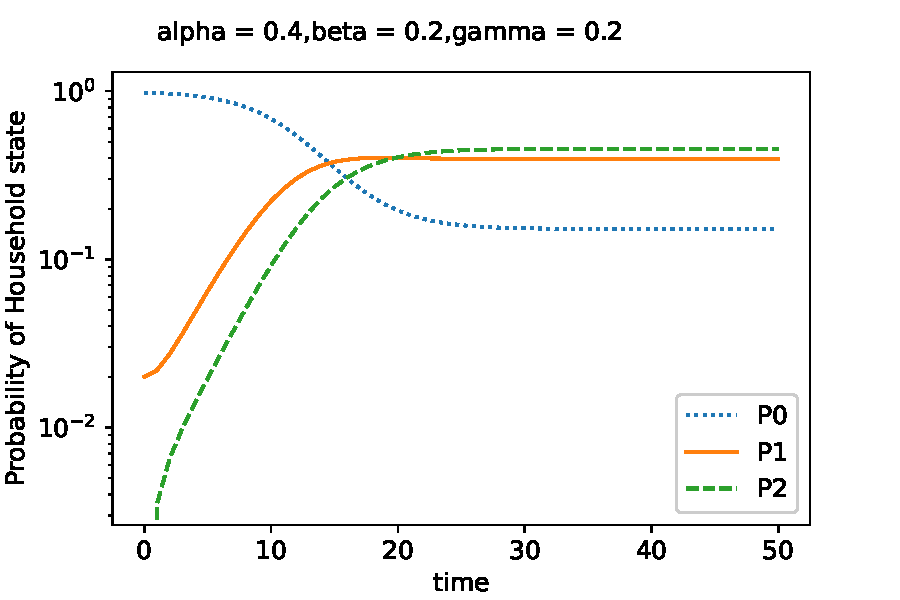
\includegraphics[width=\linewidth]{sim/01g1.pdf}
	    \caption{\(\alpha=0.4, \beta=0.2, \gamma=0.2\)}
	    \label{alpha four}
	\end{subfigure}
	\begin{subfigure}[b]{0.4\linewidth}
	    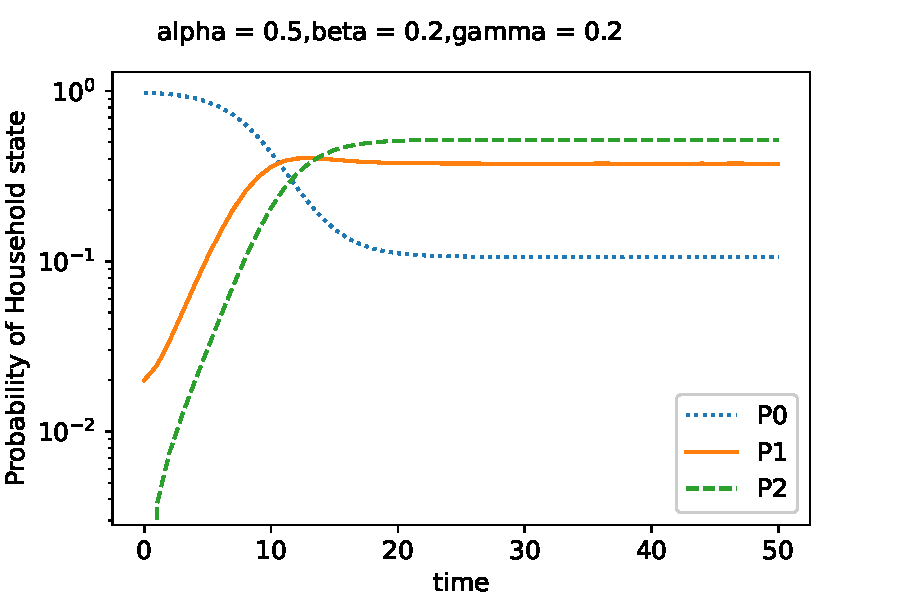
\includegraphics[width=\linewidth]{sim/021_g2.pdf}
	    \caption{\(\alpha=0.5, \beta=0.2, \gamma=0.2\)}
	    \label{alpha five}
	\end{subfigure}
	\begin{subfigure}[b]{0.4\linewidth}
	    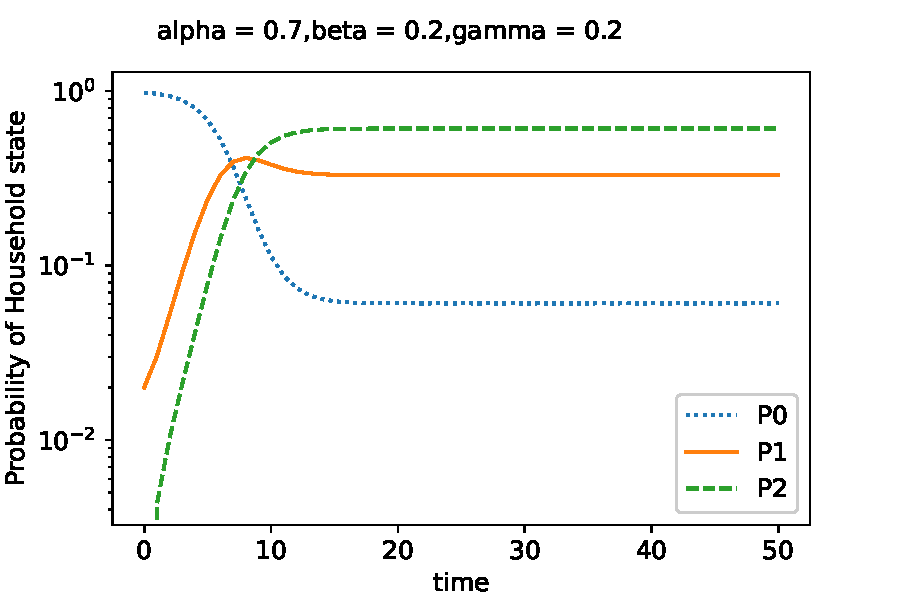
\includegraphics[width=\linewidth]{sim/031_g4.pdf}
	    \caption{\(\alpha=0.7, \beta=0.2, \gamma=0.2\)}
	    \label{alpha seven}
	\end{subfigure}
	\begin{subfigure}[b]{0.4\linewidth}
	    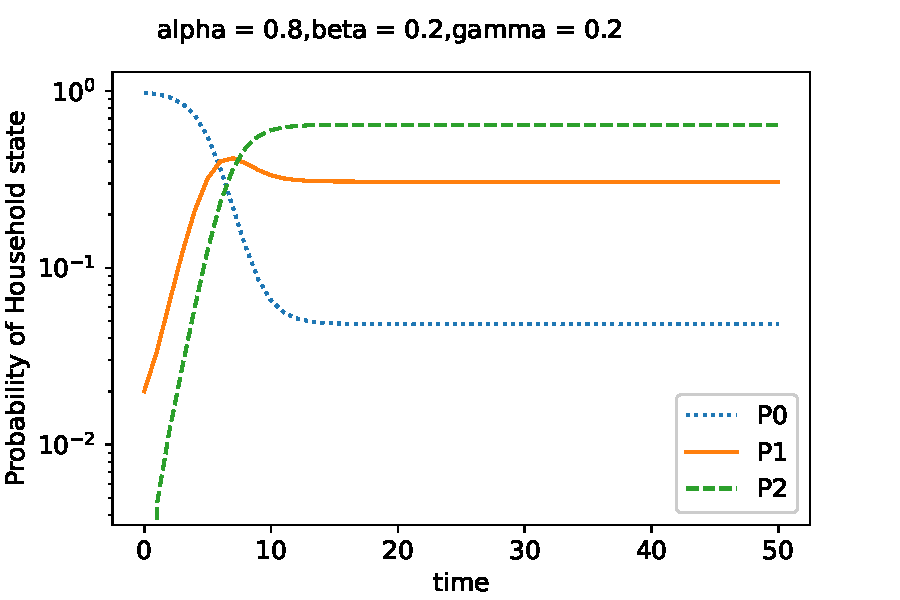
\includegraphics[width=\linewidth]{sim/041_g5.pdf}
	    \caption{\(\alpha=0.8, \beta=0.2, \gamma=0.2\)}
	    \label{alpha eight}
	\end{subfigure}
	\caption{'Probability of Household state' on $y-axis$ vs 'time' on $x-axis$ with varying $\alpha$}
	\label{fig Probabilities of Household state varying alpha}
\end{figure}


At figure \ref{fig Probabilities of Household state varying alpha} y-axis is represented by probability of household state with logarithmic scaling values and x-axis by timestep (or days) is shown to observe movement of household states. We use notation 'P0' for $P_0$ by dotted ( .. ) line, 'P1' for $P_1$ with connected line ( - ) and 'P2' by $P_2$ with dash line \( (--) \) to represent them. In figure \ref{alpha four} $ P_0 $ decreases with change with time, whereas $P_1$ increases with change with time and state $P_2$ also shows increament with time. All four graphs at \ref{fig Probabilities of Household state varying alpha} shows similar trajectories that after relative period of time all three probability of household states become steady.\\
   
In figures: \ref{fig Probabilities of Household state varying alpha}, parameters $\beta$ and $\gamma$ are kept fixed at 0.2 rate while $\alpha$ is varied at figure (a) with 0.4, figure (b) with 0.5, figure (c) with 0.7 and figure (d) with 0.8 rates to observe distinct influence of trajectories. We observed that the trajectory of $P_0$ decreases with time as rate $\alpha$ gradually increases before reaching to steady state. Similarly the trajectories of $P_1$ and $P_2$ gradually increases with time when $\alpha$ rate is increased gradually and forms crossover regions before reaching to steady state or equilbrium state. 
It is also observed that the time taken by the probability of household states to cross over each other happens in shorter duration time of gradual increase in $\alpha$ parameter.\\   
             
\par{\textbf{Steady values}}
The steady values is also studied by generating a text file from simulation. The values of each probability of household states and total infection rate \ref{Total Infection rate} in each time step are recorded. We take output values of probability of household states aligned with total infection rate. This allignment will be considered as steady state value when approximated value defined as in \ref{time step of steady values of probability}. The total infection rate is calculated using \ref{Total Infection rate}. We use notation $P_{k_{t_{i}}}$ to represent the probability of household states \( k \in \{0,1,2 \}\) values in time step '$t_{i}$' where \( i  \in \{0,1...\infty \} \).  
Equation shown below \ref{time step of steady values of probability} defines the criteria to take the values. 
\begin{equation}
\label{time step of steady values of probability}
 |P_{k_{t_{i+1}}}-P_{k_{t_{i}}}| < 10^{-3}
\end{equation} 
where $P_{k_{t_{i+1}}}$ is probability of household state values at timestep $t_{i+1}$ after one step further reaching the steady values and $P_{k_{t_{i}}}$ is the probability of household state values at time step $t_{i}$ where we reach steady state values. For example in table \ref{tab Total infection rate and total timestep reached for Probabilities of Household to reach steady states varying alpha} the values of all probabilities in household is approximately similar at $\alpha$ = 0.4 to 35th timestep.  
And for total infection rate \ref{time step of steady values of total infection} we use criteria as follows 
\begin{equation}
\label{time step of steady values of total infection}
 |I_{Total_{t_{i+1}}}-I_{Total_{{t_{i}}}}| < 10^{-3}
\end{equation} 
where $I_{Total_{t_{i+1}}}$ is total infection rate at time step $t_{i+1}$ after one step further reaching the steady values and $I_{Total_{t_{i}}}$ is the total infection rate at time step $t_{i}$ where we reach steady state values.
Total infection rate \ref{Total Infection rate} and total recovery rate \ref{Total Recovered rate} values  with varying $\alpha$ are shown below in \ref{tab Total infection rate and total timestep reached for Probabilities of Household to reach steady states varying alpha} 

\begin{table}[H]
	\centering 
	\caption{Total infection rate, Total recovered rate and time step taken by probabilities of household state to reach steady states with varying $\alpha$}
	\label{tab Total infection rate and total timestep reached for Probabilities of Household to reach steady states varying alpha}
	\begin{tabular}{cccccc}
	\toprule
     Name & $\alpha$ = 0.4  & $\alpha$ = 0.5 & $\alpha$ = 0.6 & $\alpha$ = 0.7 & $\alpha$ = 0.8 \\
     \midrule
     Total infection rate ($I_{Total}$) & (1.290) & (1.402) & (1.482) & (1.543) & (1.592) \\
     Total recovered rate ($R_{Total}$) & (0.258) & (0.280) & (0.296) & (0.308) & (0.318) \\
	 Total Timestep & (35) & (28) & (26) & (23) & (19) \\
	\bottomrule
	\end{tabular}
\end{table}

We notice in table \ref{tab Total infection rate and total timestep reached for Probabilities of Household to reach steady states varying alpha} that total infection rate and total recovered rate increases when $\alpha$ rate gradually increases while time taken to reach steady state decreases. After calculating total infection rate values we will show results of probability of household states distribution in table \ref{tab Probability of Household state values varying alpha}. 

\begin{table}[H]
	\centering 
	\caption{Simulation : Probability of household state values with varying $\alpha$}
	\label{tab Probability of Household state values varying alpha}
	\begin{tabular}{cccccc}
	\toprule
     Probabilities of household states & $\alpha$ = 0.4  & $\alpha$ = 0.5 & $\alpha$ = 0.6 & $\alpha$ = 0.7 & $\alpha$ = 0.8 \\
     \midrule
	 $P_0$ & 0.151  & 0.106 & 0.078 & 0.060  & 0.048 \\
	 $P_1$ & 0.394  & 0.375 & 0.351 & 0.328  & 0.307 \\
	 $P_2$ & 0.453  & 0.518 & 0.569 & 0.610  & 0.644 \\
	\bottomrule
	\end{tabular}
\end{table}
We observed that the steady state values from \ref{tab Probability of Household state values varying alpha} in $P_0$ decreases from 0.151 till 0.048 with increased $\alpha$ rates. Similarly the values of $P_1$ also decreases from 0.394 till 0.307 gradually in similar trend but $P_2$ values increases from 0.453 to 0.644 with gradual increase in $\alpha$ rate.
We use graph \ref{discrete alpha values} below to show probabilities of household states values with varying rates of $\alpha$ in table \ref{tab Probability of Household state values varying alpha}. 

\begin{figure}[H]
\centering
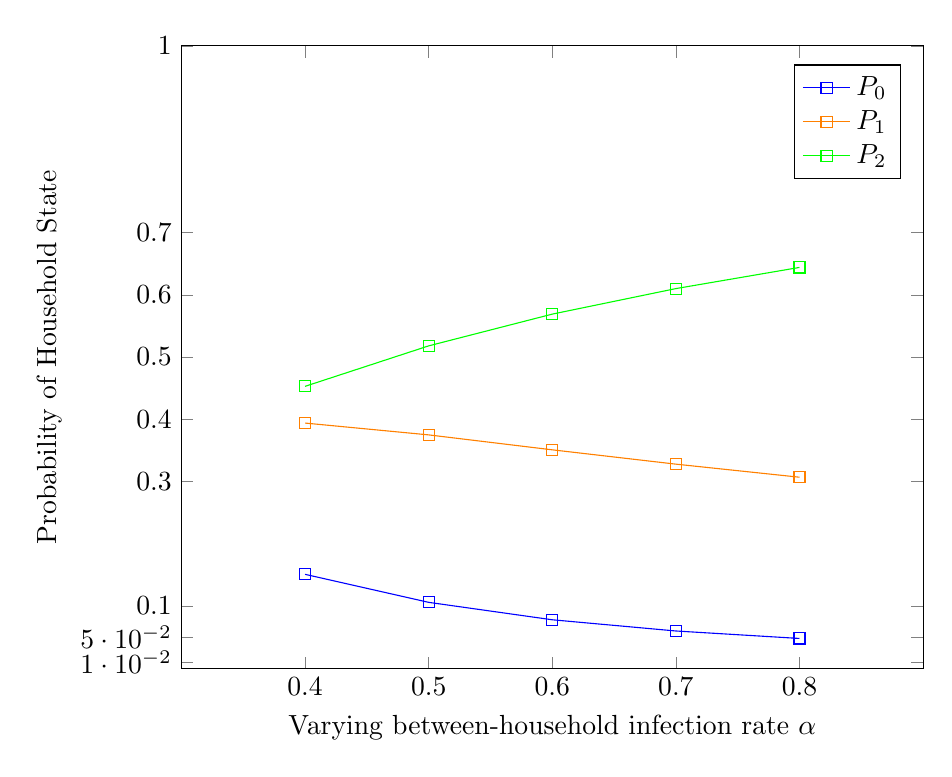
\begin{tikzpicture}
\begin{axis}[
    xlabel={ Varying between-household infection rate $\alpha$ },
    ylabel={Probability of Household State},
    xmin=0.3, xmax=0.9,
    ymin=0, ymax=1,
    xtick={0.4, 0.5, 0.6, 0.7, 0.8},
    ytick={0.01, 0.05, 0.1, 0.3, 0.4,0.5,0.6,0.7,1.0},
    legend pos=north east,
]
\addplot[color=blue,mark=square] coordinates {
				(0.4, 0.151)
    				(0.5, 0.106)
    				(0.6, 0.078)
    				(0.7, 0.060)
    				(0.8, 0.048)
};
\addplot[color=orange,mark=square] coordinates {
                (0.4, 0.394)
                (0.5, 0.375)
                (0.6, 0.351)
                (0.7, 0.328)
                (0.8, 0.307)
};
\addplot[color=green,mark=square] coordinates {
                (0.4, 0.453)
                (0.5, 0.518)
                (0.6, 0.569)
                (0.7, 0.610)
                (0.8, 0.644)
};
\legend{$P_0$,$P_1$,$P_2$}
\end{axis}
\end{tikzpicture}
\caption{'Probability of Household State' on $x-axis$ vs 'Varying between-household infection rate $\alpha$' on $y-axis$ }
\label{discrete alpha values}
\end{figure}
In figure \ref{discrete alpha values} the values of $P_0$ and $P_1$ decreases with gradual increase in between-household infection rate $\alpha$ while value of '$P_2$' decreases.      

\subsection*{Influence of within-household infection rate on Master Equation}
\label{observation beta parameter}
In this section, we show figures of $\beta$'s influence in Master Equations in  figure :\ref{fig Probability of Household state values varying beta} and figure \ref{discrete beta values}. We will also show two tables of steady state values of total infection rate in table : \ref{tab Total infection rate and timestep reached for Probabilities of Household to reach steady states varying beta} and probability of household states in table : \ref{table Household state values varying beta} of $\beta$'s influence in Master Equation. 

	\begin{figure}[H]
	\centering
	\begin{subfigure}[b]{0.4\linewidth}
	  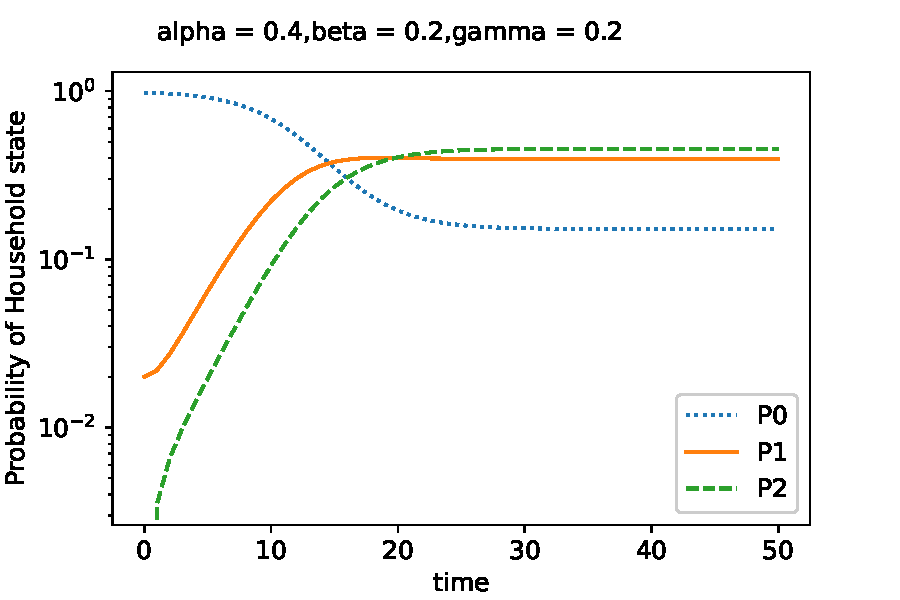
\includegraphics[width=\linewidth]{sim/01g1.pdf}
	  \caption{\(\alpha=0.4, \beta=0.2, \gamma=0.2\)}
	  \label{beta two}
	\end{subfigure}
	\begin{subfigure}[b]{0.4\linewidth}
	  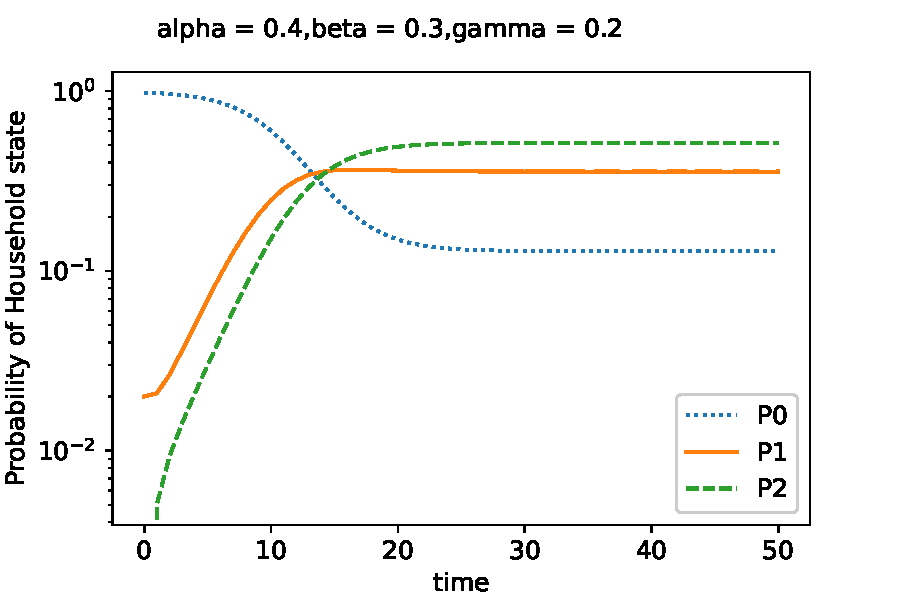
\includegraphics[width=\linewidth]{sim/022_g6.pdf}
	  \caption{\(\alpha=0.4, \beta=0.3, \gamma=0.2\)}
	  \label{beta three}
	\end{subfigure}
	\begin{subfigure}[b]{0.4\linewidth}
      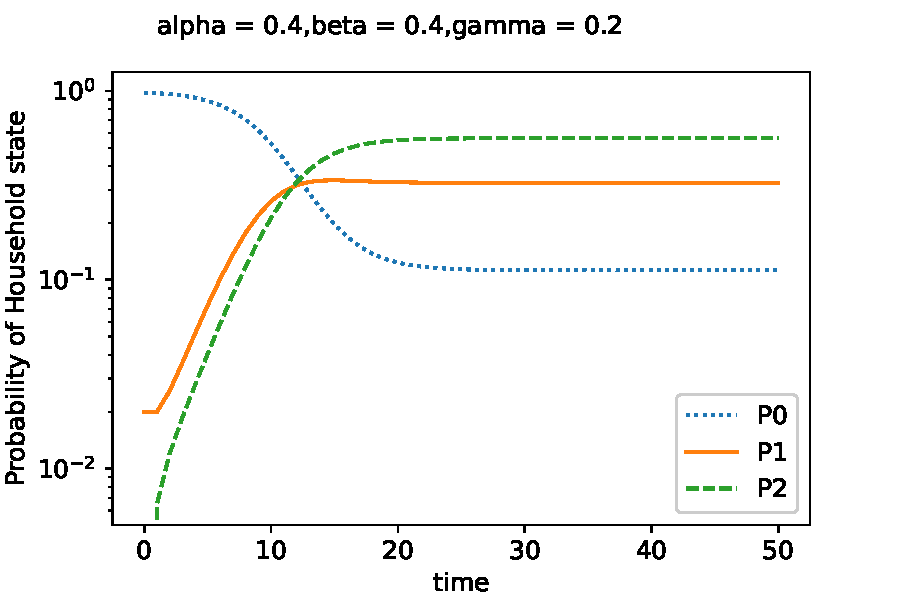
\includegraphics[width=\linewidth]{sim/032_g11.pdf}
	  \caption{\(\alpha=0.4, \beta=0.4, \gamma=0.2\)}
	  \label{beta four}
	\end{subfigure}
	\begin{subfigure}[b]{0.4\linewidth}
	  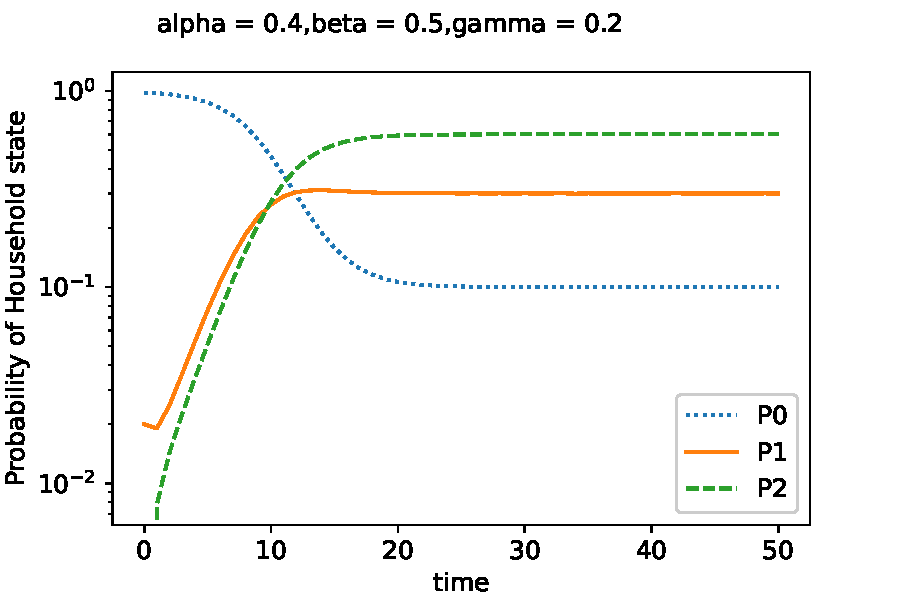
\includegraphics[width=\linewidth]{sim/042_g16.pdf}
	  \caption{\(\alpha=0.4, \beta=0.5, \gamma=0.2\)}
	  \label{beta five}
	\end{subfigure}
	\caption{''Probability of Household state' on $y-axis$ vs 'time' on $x-axis$ with varying $\beta$}
	\label{fig Probability of Household state values varying beta}
	\end{figure}
	
We plot figures \ref{fig Probability of Household state values varying beta} to observe within-household infection rate $\beta$ influence on Master equations and vary it at figure (a) with 0.2, figure (b) with 0.3, figure (c) with 0.4, figure (d) with 0.5 while fixing $\alpha$ constant at 0.4 and $\gamma$ constant at 0.2. We observed that all probability of household states reaches to steady states. In addition, we observe that gradually increasing $\beta$ in figures \ref{fig Probability of Household state values varying beta} shows the path of trajectories decreases in $P_0$ but increases in $P_1$ and $P_2$ before eventually reaching to steady paths.\\  
The table shown below is steady values of the total infection rate and total recovery rate and their timestep to reach steady state are shown in \ref{tab Total infection rate and timestep reached for Probabilities of Household to reach steady states varying beta}.
 
\begin{table}[H]
	\centering 
	\caption{Total infection rate, Total recovered rate and time step taken by probabilities of household state to reach steady states varying $\beta$}
	\label{tab Total infection rate and timestep reached for Probabilities of Household to reach steady states varying beta}
	\begin{tabular}{ccccc}
	\toprule
     Name & $\beta$ = 0.2  & $\beta$ = 0.3 & $\beta$ = 0.4 & $\beta$ = 0.5 \\
     \midrule
     Total infection rate ($I_{Total}$) & (1.290) & (1.375) & (1.441) & (1.493) \\
     Total recovered rate ($R_{Total}$) & (0.258) & (0.275) & (0.288) & (0.298) \\
	 Timestep & (35) & (31) & (30) & (27) \\
	\bottomrule
	\end{tabular}
\end{table}

In table : \ref{tab Total infection rate and timestep reached for Probabilities of Household to reach steady states varying beta} we observe that both total infection rate and total recoverd rate increases in values when the value of $\beta$ is gradually increased and the time duration taken by household states to reach steady state values gradually decreases. 
We show below probability of Household state values varying beta:
\begin{table}[H]
	\centering 
	\caption{Simulation : Probability of household state values with varying $\beta$}
	\label{table Household state values varying beta}
	\begin{tabular}{ccccc}
	\toprule
     Probability of HouseHold state & $\beta$ = 0.2 & $\beta$ = 0.3  & $\beta$ = 0.4 & $\beta$ = 0.5 \\
     \midrule
	 $P_0$ & 0.151 & 0.128  & 0.112  & 0.100 \\
	 $P_1$ & 0.394 & 0.356  & 0.325  & 0.299 \\
	 $P_2$ & 0.453 & 0.514  & 0.561  & 0.599 \\
	\bottomrule
	\end{tabular}
\end{table}

We observe from the table \ref{table Household state values varying beta} influence of gradual increase in $\beta$ decreases the steady state values of $P_0$ and $P_1$ but $P_2$ values in steady states gets increased. We show the figure \ref{discrete beta values}.   
\begin{figure}[H]
\centering 
	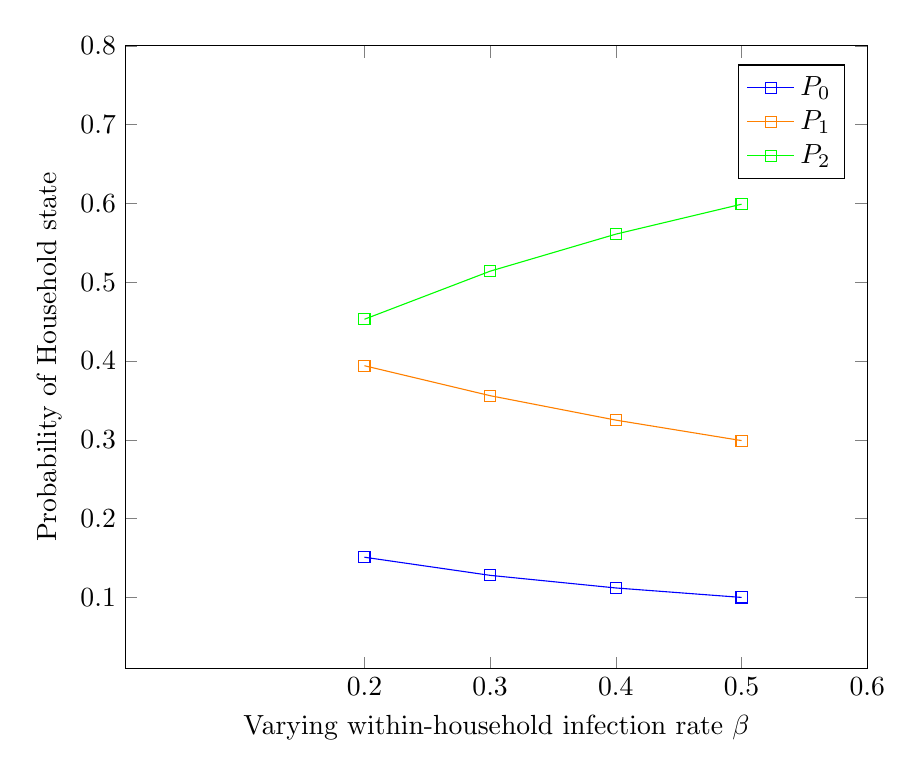
\begin{tikzpicture}
	\begin{axis}[
    xlabel={Varying within-household infection rate $\beta$},
    ylabel={Probability of Household state},
    xmin=0.01, xmax=0.6,
    ymin=0.01, ymax=0.8,
    xtick={0.2, 0.3, 0.4, 0.5, 0.6, 0.7 },
    ytick={0.1,0.2,0.3,0.4,0.5,0.6, 0.7, 0.8},
    legend pos=north east,
]
\addplot[color=blue,mark=square] coordinates {
				(0.2, 0.151)
				(0.3, 0.128)
    				(0.4, 0.112)
    				(0.5, 0.100)
};
\addplot[color=orange,mark=square] coordinates {
                (0.2, 0.394)
                (0.3, 0.356)
                (0.4, 0.325)
                (0.5, 0.299)
};
\addplot[color=green,mark=square] coordinates {
                (0.2, 0.453)
                (0.3, 0.514)
                (0.4, 0.561)
                (0.5, 0.599)
};
\legend{$P_0$,$P_1$,$P_2$}
\end{axis}
\end{tikzpicture}
\caption{'Probability of Household State' on $x-axis$ vs 'Varying within-household infection rate $\beta$' on $y-axis$}
\label{discrete beta values}
\end{figure}
In figure \ref{discrete beta values} it is clearly seen that $P_1$ and $P_0$ decreases with gradual increase in $\beta$ but $P_2$ increases. 
\subsection*{Influence of household recovery rate on Master Equation}
\label{observation gamma parameter} 
In previous sections we discussed about gradual change in $\alpha$ and $\beta$ on master equation now we will observe at the recovery parameter $\gamma$'s influence on master equation in this section. 

\begin{figure}[H]
 \centering
	\begin{subfigure}[b]{0.4\linewidth}
	  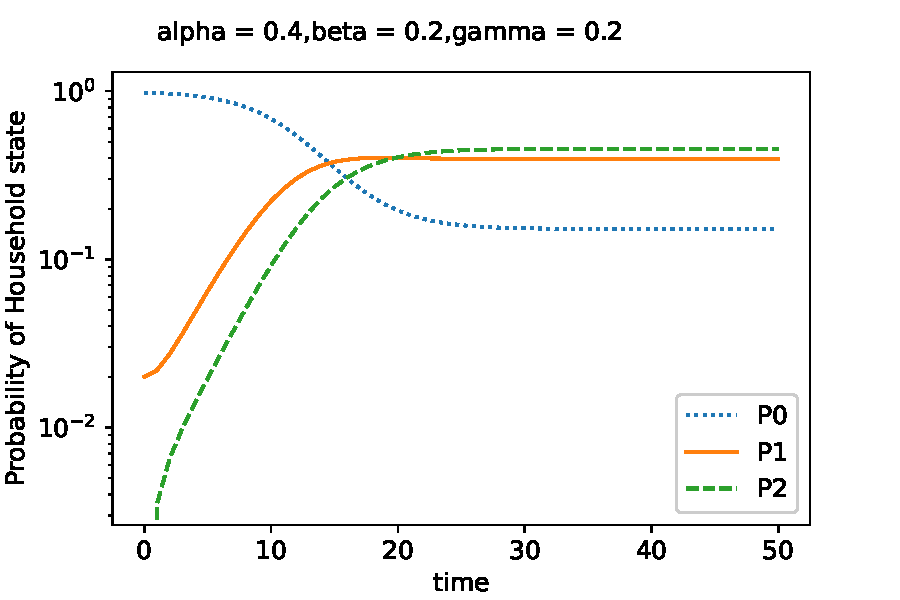
\includegraphics[width=\linewidth]{sim/01g1.pdf}
	  \caption{\(\alpha=0.4, \beta=0.2, \gamma=0.2\)}
	  \label{gamma two }
	\end{subfigure}
	\begin{subfigure}[b]{0.4\linewidth}
	  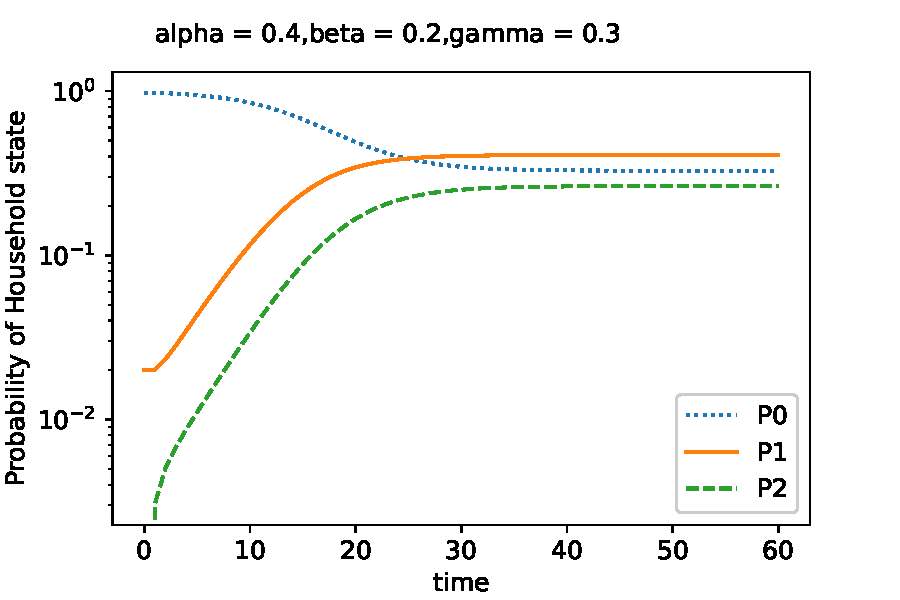
\includegraphics[width=\linewidth]{sim/023_b6.pdf}
	  \caption{\(\alpha=0.4, \beta=0.2, \gamma=0.3\)}
	  \label{gamma three}
	\end{subfigure}
	\begin{subfigure}[b]{0.4\linewidth}
	  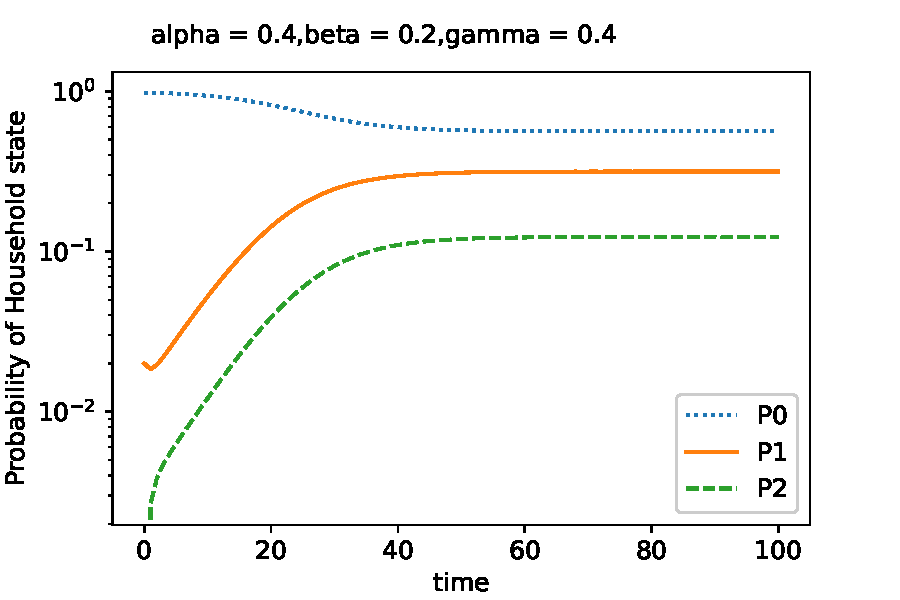
\includegraphics[width=\linewidth]{sim/033_a1.pdf}
	  \caption{\(\alpha=0.4, \beta=0.2, \gamma=0.4\)}
	  \label{gamma four}
	\end{subfigure}
	\begin{subfigure}[b]{0.4\linewidth}
	  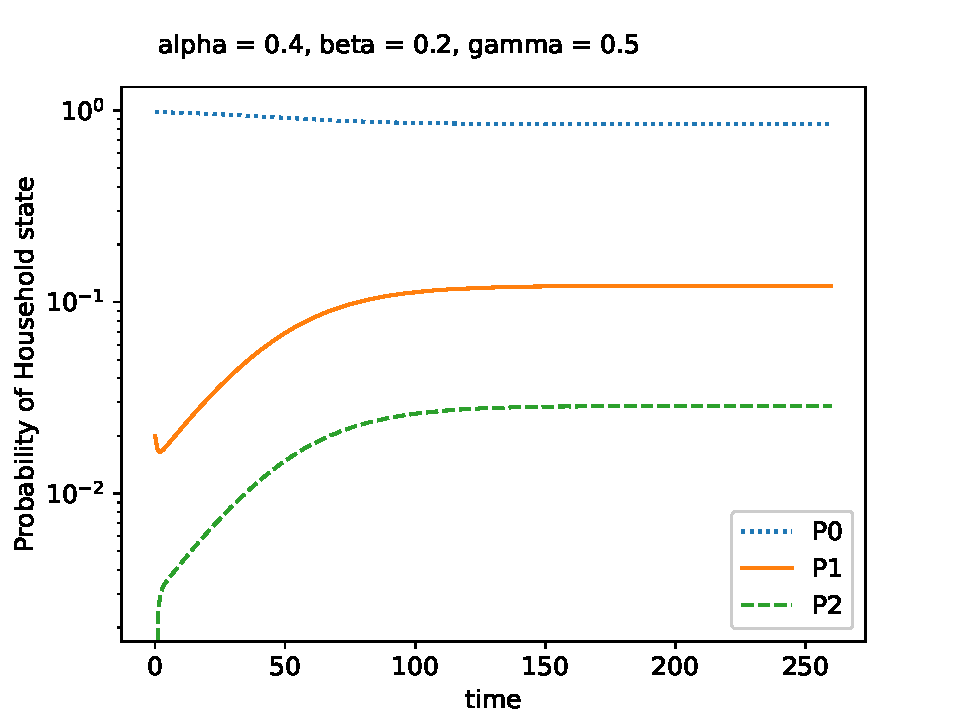
\includegraphics[width=\linewidth]{sim/033_a2_5.pdf}
	  \caption{\(\alpha=0.4, \beta=0.2, \gamma=0.5\)}
	  \label{gamma five}
	\end{subfigure}
	\begin{subfigure}[b]{0.4\linewidth}
	  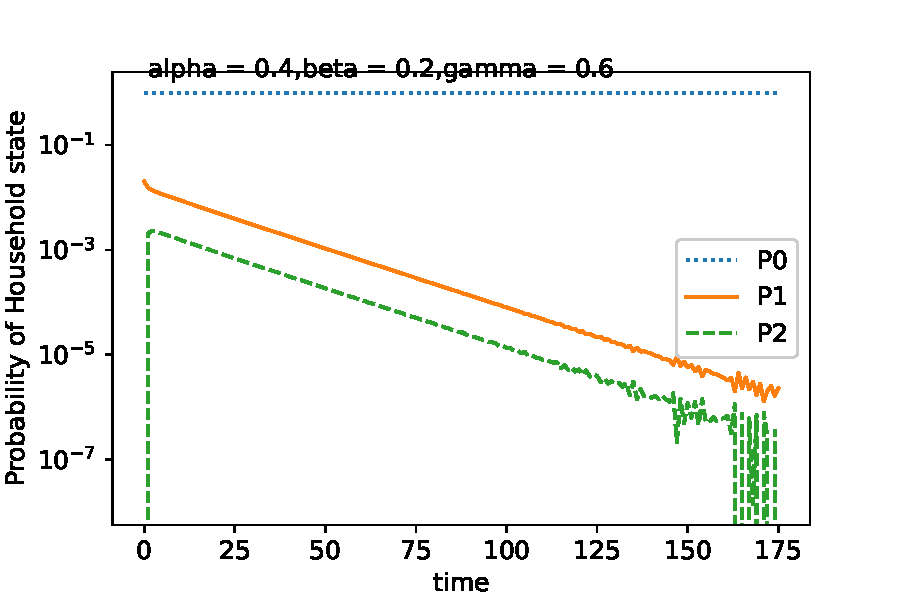
\includegraphics[width=\linewidth]{sim/043_a3.pdf}
	  \caption{\(\alpha=0.4, \beta=0.2, \gamma=0.6\)}
	  \label{gamma six}
	\end{subfigure}
	\caption{'Probability of Household state' on $y-axis$ vs 'time' on $x-axis$ with varying $\gamma$}
	\label{fig changing gamma values}
\end{figure}

We observe an steady states in trajectories figure (a),(b), (c) and (d) in figure \ref{fig changing gamma values} but unstable trajectories in figure (e) when $\gamma$ is gradually increased. In figure (a),(b) and (c) of figure \ref{fig changing gamma values}, the timesteps taken by trajectories to reach steady states increases when $\gamma$ increases. We can also observe values of total infected rate and total recovered rate in table \ref{tab Total infection rate and days reached for Probabilities of Household to reach steady states varying gamma}.
Our observation of total infection rate and the criteria to take time steps referred from equation \ref{time step of steady values of total infection} to reach steady values or unsteady states are shown in table : \ref{tab Total infection rate and days reached for Probabilities of Household to reach steady states varying gamma} 
 
\begin{table}[H]
	\centering 
	\caption{Total infection rate, Total recovered rate and time step taken by probabilities of household state to reach steady states varying $\gamma$}
	\label{tab Total infection rate and days reached for Probabilities of Household to reach steady states varying gamma}
	\begin{tabular}{ccccc}
	\toprule
     Name & $\gamma$ = 0.3 & $\gamma$ = 0.4 & $\gamma$ = 0.5 & $\gamma$ = 0.6 \\
     \midrule
     Total infection rate ($I_{Total}$) & (0.922) & (0.545) & (0.161) & - \\
     Total recovered rate ($I_{Total}$) & (0.276) & (0.218) & (0.080) & - \\
	 Timestep & (54) & (74) & (185) & - \\
	\bottomrule
	\end{tabular}
\end{table}

These steady state criteria values from table \ref{tab Total infection rate and days reached for Probabilities of Household to reach steady states varying gamma} are used to show the values of probability household states below table \ref{Probability of Household state values with varying gamma}. In table \ref{tab Total infection rate and days reached for Probabilities of Household to reach steady states varying gamma} the steady state values in total infection rate sharply decreases as gradual increase in recovery rate while in total recovery rate slightly increases in $\gamma$ = 0.3 but sharply decreases from $\gamma$ = 0.4 onwards till approximately 0.5 and then it starts to show unsteady values or reach negligible to zero. The time step taken by total infection rate to reach steady state increases in gradual increase of recovery rate till $\gamma$ = 0.5. At $\gamma$ = 0.6, $P_0$ and $P_1$ reaches to negligible to zero. The household states values aligned with total infection rate is shown in table \ref{Probability of Household state values with varying gamma}.


\begin{table}[H]
	\centering 
	\caption{Simulation : Probability of household state values varying $\gamma$}
	\label{Probability of Household state values with varying gamma}
	\begin{tabular}{ccccccc}
	\toprule
     Probability of Household state & $\gamma$ = 0.3  & $\gamma$ = 0.4 & $\gamma$ = 0.5 & $\gamma$ = 0.6 \\
     \midrule
	 $P_0$ & 0.327  & 0.561  & 0.849 & 0.9999  \\
	 $P_1$ & 0.408  & 0.315  & 0.121 & -\\%(5.95)^{-5} \\
	 $P_2$ & 0.264  & 0.123  & 0.028 & -\\%(9.56)^{-06} \\
	\bottomrule
	\end{tabular}
\end{table}

We observe in \ref{Probability of Household state values with varying gamma} that in household state $P_0$ the equilibrium values increases sharply in gradual increase in recovery parameter. For $P_1$ there is slight increase in recovery rate from 0.2 to 0.3 but gets decreases significantly from 0.4 till 0.5 while for $P_2$ there is significant decrease till 0.5. At $\gamma$ 0.6 the values of $P_1$ and $P_2$ is negligible to zero. The probability household states values gradual increase of recovery rate is shown in \ref{discrete gamma values }.    
%table showing discrete 
\begin{figure}[H]
\centering
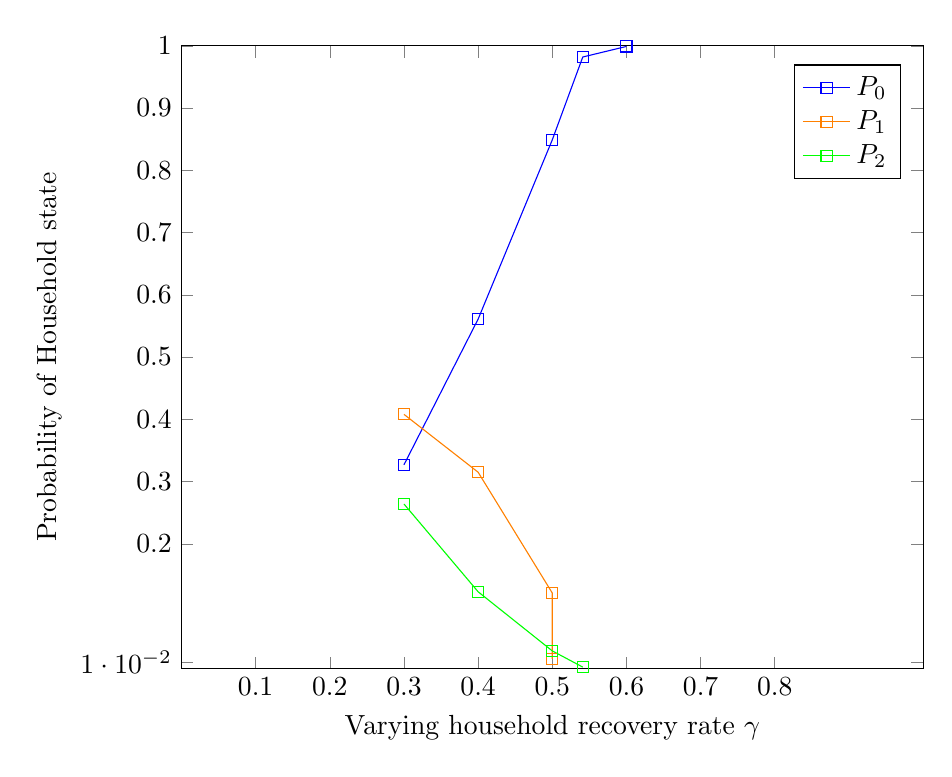
\begin{tikzpicture}
\begin{axis}[
    xlabel={ Varying household recovery rate $\gamma$},
    ylabel={Probability of Household state},
    xmin=0, xmax=1,
    ymin=0, ymax=1,
    xtick={0.1, 0.2, 0.3, 0.4, 0.5, 0.6, 0.7, 0.8},
    ytick={0.01, 0.2, 0.3, 0.4, 0.5, 0.6, 0.7, 0.8, 0.9, 1.0},
    legend pos=north east,
]
\addplot[color=blue,mark=square] coordinates {
				(0.3, 0.327)
    				(0.4, 0.561)
    				(0.5, 0.849)
    				(0.5411, 0.982)
    				(0.6, 0.999)
};
\addplot[color=orange,mark=square] coordinates {
				(0.3, 0.408)
    				(0.4, 0.315)
    				(0.5, 0.121)
    				(0.5, 0.015)
    				%(0.6, )%5.95^{10^{-5}}
};
\addplot[color=green,mark=square] coordinates {
				(0.3, 0.264)
    				(0.4, 0.123)
    				(0.5, 0.028)
    				(0.5411, 0.002)
    				%(0.6, )%9.95^{10^{-5}}
};
\legend{$P_0$,$P_1$,$P_2$}
\end{axis}
\end{tikzpicture}
\caption{'Probability of Household State' on $x-axis$ vs 'Varying household recovery rate $\gamma$' on $y-axis$ }
\label{discrete gamma values }
\end{figure}

We can see in above \ref{discrete gamma values } that $P_0$ state sharply rises but $P_1$ and $P_2$ falls down reaching stage reaching negligible to zero in timesteps towards infinity.

\section{Analysis of Numerical Results in Equilibrium }
\subsection{Analysis of Disease-Free Equilibrium(DFE)}
With cases observed in 'Analysis of Eigenvalue for DFE' in analytical section of DFE, we show a figure to observe stable regions and instable regions for DFE in master equation SHH of size two. We take our intial parameter $\alpha$ being constant at 0.4 and set range of parameters $\beta$ and $\gamma$ from 0.1 to 1 dividing each by 1000. This is done in order to give smooth separation of regions to make a distinction of stable and unstable regions between gamma in y-axis and beta in x-axis. Each values given in $\alpha$, $\beta$ and $\gamma$ represent trace values in \ref{Trace} and determinant values in \ref{Determinant}. The calculation of eigenvalue in both equation at \ref{eigenvalue} resulted in figure \ref{regions of stability and unstability}. According to the cases discussed in section 'Analysis of eigenvalues for DFE', we set up equation  \ref{eigenvalue} such that if both eigenvalues are negative then we show stable region which is denoted by color blue and if anyone of the eigenvalues is positive then the regions are unstable which is denoted by color red.

\begin{figure}[H]
  \centering
  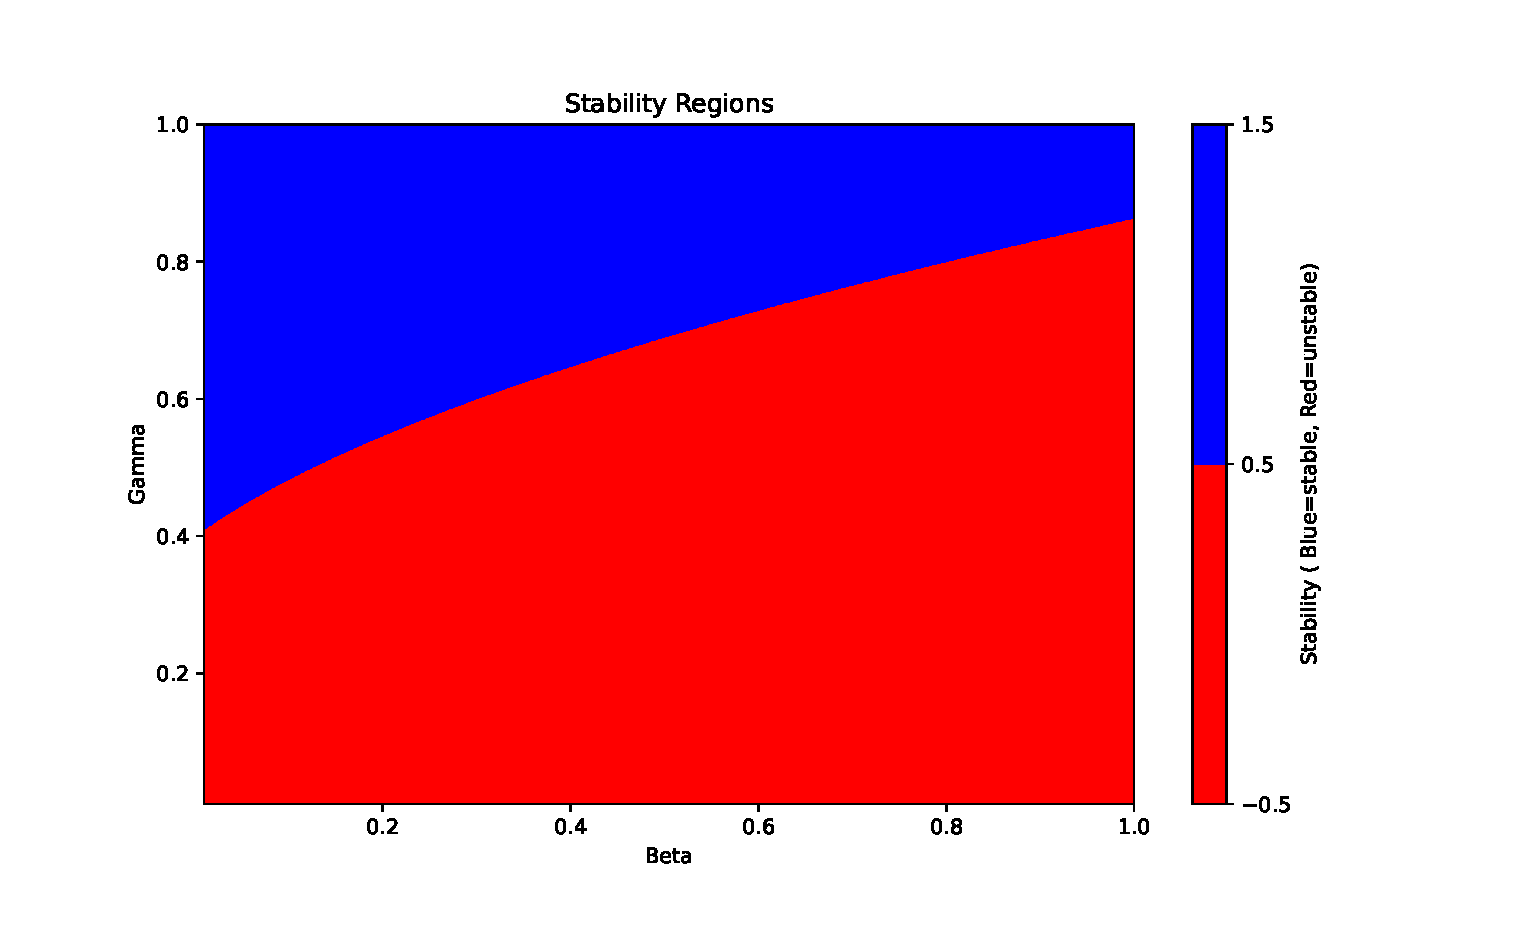
\includegraphics[height=7cm]{graph/stability.eps}
  \caption{'Gamma'($\gamma$) as recovery rate on $y-axis$ and 'Beta'($\beta$) as within-household infection rate on $x-axis$ with constant alpha($\alpha$) as between-household infection rate' at 0.4.}
  \label{regions of stability and unstability}
\end{figure}
Figure \ref{regions of stability and unstability} shows stable regions and unstable regions in disease-free equilibrium of SHH of size two.\\ 
The discussion of equilibrium case in disease-free equilibrium is as follows. 
\paragraph*{case : $ Tr < 0$ and $Tr > \sqrt{Tr^2-4D} $ , where  $D > 0$ and $Tr^2 > 4D $}:

In this case we use term $ Tr < 0 $, which interchangeably means \( \alpha < \beta + 3\gamma \) and $ D > 0 $ which means \( \alpha < \frac{\gamma^2}{\beta + \gamma} \). In this case, when $ Tr < 0 $ and $Tr > \sqrt{Tr^2-4D} > 0$ with $D > 0$ and $ Tr^2-4D > 0 $, it shows the stable region because both eigenvalues   are negative in \ref{eigenvalue} and for other cases, it shows unstable regions in \ref{regions of stability and unstability}. We limit our study to real eigenvalues and complex pair of eigenvalues are neglected. The $\alpha$ parameter has to be strictly less than ($\beta$ + $3\gamma$) in $ Tr < 0$ and for $D > 0$ in \ref{Determinant} to be positive. To fulfill the condition stated earlier, it is necessary for the value of $\beta$  of \( \alpha < \frac{\gamma^2}{\beta + \gamma} \) to be lower than $\gamma$. A higher rate of $\gamma$ results in stable regions. This means higher recovery rate is needed for disease-free equilibrium. And the solution near the equilibrium point 
will result into stability. For example, if $\beta$ is zero, $\gamma$ is greater than 0.4 and $\alpha$ is 0.4 then the region is stable. Following up with previous example, to satisfy $Tr$ condition the recovery rate has to be higher with (3$\gamma$). Also the difference of infection rates ($\alpha - \beta$) has to lower greater than (3$\gamma$) . Only the higher recovery rates will make region stable. This case with $D > 0$ is significant criteria for $\gamma$ to be high. This scenario is also seen in above figure. 
The other cases explored resulted in unstable region when \( \alpha > \beta + 3\gamma \) and \( \alpha > \frac{\gamma^2}{\beta + \gamma} \) i.e with betwee-household infection rates leading to unstable in DFE.  

\subsection{Analysis of Endemic Equilibrium(EE)}
In section, we substitute the equations \ref{positive root of P0}, \ref{positive root of P1} and \ref{positive root P2} with parameters $\alpha$, $\beta$ and $\gamma$ as shown in table \ref{tab Probability of Household state values varying alpha}, \ref{table Household state values varying beta} and \ref{Probability of Household state values with varying gamma} which shows the following results. 

\textbf{Probability of household states values with varying $\alpha$}: \\
We take the rates of $\alpha$, $\beta$ and $\gamma$ from table \ref{tab Probability of Household state values varying alpha} and use them to find the solution of $P_0$ in equation \ref{positive root of P0}, $P_1$ in equation \ref{positive root of P1} and $P_2$ in equation \ref{positive root P2}. We get the following results in table : \ref{root table Household state values varying alpha}
\begin{table}[H]
	\centering 
	\caption{Equilibrium : Probability of household states values with varying $\alpha$}
	\label{root table Household state values varying alpha}
	\begin{tabular}{cccccc}
	\toprule
     HouseHold states & $\alpha$ = 0.4  & $\alpha$ = 0.5 & $\alpha$ = 0.6 & $\alpha$ = 0.7 & $\alpha$ = 0.8 \\
     \midrule
	 $P_0$ & 0.151  & 0.106  & 0.078  & 0.060  & 0.048 \\
	 $P_1$ & 0.394  & 0.375  & 0.351  & 0.328  & 0.307 \\
	 $P_2$ & 0.454  & 0.518  & 0.569  & 0.610  & 0.644 \\
	\bottomrule
	\end{tabular}
\end{table}
We compared the values of simulation in Runge-Kutta method: \ref{tab Total infection rate and total timestep reached for Probabilities of Household to reach steady states varying alpha} with endemic equilibrium values in table \ref{root table Household state values varying alpha} and found them to be approximately similar.\\ 
Referencing equation \ref{positive root of P0}, we gradually increase $\alpha$ but keep the other two parameters fixed. The increase in $\alpha$ rate of equation \ref{positive root of P0}  decreases the value of $P_0$ while sum of between-household and within-household infection rate $(\alpha + \beta)$ in \ref{positive root of P0} should not make much difference. This decreases the value of $P_0$ by $\alpha$ in $\frac{\gamma}{2\alpha\beta}$ in equation \ref{positive root of P0} which have direct impact on $P_0$ and \( (1-P_0) \) in equation \ref{positive root of P1}. The decrease in $P_0$ increases the value of $P_1$ at \ref{positive root of P1}. The recovery rate remains constant in the \( \gamma + \alpha P_0 \) and the $\alpha P_0$ term reduces the output in $P_1$. In equation \ref{positive root P2}, $P_2$ depends on the values of $P_1$ and $P_0$. The accumulation of low values of $P_1$ and $P_0$ leads to a high value of $P_2$. Therefore, it can be concluded that a gradual increase in the rate of $\alpha$ results in an increase in value of $P_2$ and in $P_1$.\\
For each rate, we computed the eigenvalues using the values at the endemic equilibrium point and also determined the Jacobian as per Equation \ref{jacobian at endemic equilibrium point}. Our analysis revealed three eigenvalues, with one being zero and the other two being negative, indicating stable regions as possibility of endemic equilibrium. The gradual increase in the between-household infection rate resulted in a reduction of negative eigenvalues.\\ 

\textbf{Probability of household states values with varying $\beta$}: \\
We take the rates of $\alpha$, $\beta$ and $\gamma$ from table \ref{table Household state values varying beta} and use them to find the solution of $P_0$ in equation \ref{positive root of P0}, $P_1$ in equation \ref{positive root of P1} and $P_2$ in equation \ref{positive root P2}. We get the following results in table : \ref{root table Household state values varying beta}
\begin{table}[H]
	\centering 
	\caption{Equilibrium : Probability of household states values with varying $\beta$}
	\label{root table Household state values varying beta}
	\begin{tabular}{ccccc}
	\toprule
     HouseHold states & $\beta$ = 0.2 & $\beta$ = 0.3  & $\beta$ = 0.4 & $\beta$ = 0.5 \\
     \midrule
	 $P_0$ & 0.151 & 0.128  & 0.112  & 0.100 \\
	 $P_1$ & 0.394 & 0.356  & 0.325  & 0.300 \\
	 $P_2$ & 0.454 & 0.514  & 0.561  & 0.600 \\
	\bottomrule
	\end{tabular}
\end{table}
In this section we observe the effect of $\beta$ on endemic equilibrium, we compared the values of table from simulation in Runge-Kutta method: \ref{table Household state values varying beta} with endemic equilibrium values in table \ref{root table Household state values varying beta} and found them to be apporximately similar.\\ 
In table \ref{root table Household state values varying beta}, the gradual increase in $\beta$ rate equation \ref{positive root of P0} decreases the value of $P_0$. The decrease in value of $P_0$ increases $P_1$ in \ref{positive root of P1} but without direct influence of $\beta$ in \ref{positive root of P1}. In equation \ref{positive root P2}, $P_2$ depends on the values of $P_1$ and $P_0$. The sum of low values of $P_1$ and $P_0$ resulted in high values of $P_2$. We can see that the gradual increase in $\beta$ rate increases value of $P_2$ in table \ref{root table Household state values varying beta}.\\    
We calculated the eigenvalues from $\beta$ rates with endemic equlibrium solution or fixed point and from equation \ref{jacobian at endemic equilibrium point}. We find three eigenvalues in which one eigenvalue is zero and the  other two eigenvalues are negative which leads to stability which also shows possibility of endemic equilibrium. The gradual increase in the between-household infection rate decreases the negative eigenvalues.\\ 

\textbf{Probability of household states values with varying $\gamma$}: \\
We take the rates of $\alpha$, $\beta$ and $\gamma$ from table \ref{table Household state values varying beta} and use them to find the solution of $P_0$ in equation \ref{positive root of P0}, $P_1$ in equation \ref{positive root of P1} and $P_2$ in equation \ref{positive root P2}. We get the following results in table : \ref{root Household state values varying gamma}. 

\begin{table}[H]
	\centering 
	\caption{Equilibrium : Probability of household states values with varying $\gamma$}
	\label{root Household state values varying gamma}
	\begin{tabular}{cccccc}
	\toprule
     HouseHold states & $\gamma$ = 0.3  & $\gamma$ = 0.4 & $\gamma$ = 0.5 & $\gamma$ = 0.5411 & $\gamma$ = 0.6 \\
     \midrule
	 $P_0$ & 0.327  & 0.561  & 0.849 & 0.982 & - \\ %1.18
	 $P_1$ & 0.408  & 0.315  & 0.121 & 0.014 & - \\ %(-0.16)
	 $P_2$ & 0.263  & 0.123  & 0.028 & 0.002 & - \\ %(-0.02)
	\bottomrule
	\end{tabular}
\end{table}
In this section we observe the effect of $\gamma$ on endemic equilibrium, we compared the values of table from simulation in Runge-Kutta method: \ref{Probability of Household state values with varying gamma} with endemic equilibrium values in table \ref{root Household state values varying gamma} and found them to be approximately similar.\\
In table \ref{root Household state values varying gamma}, the gradual increase in recovery parameter $\gamma$ is observed from equation \ref{positive root of P0}. The increase of $\gamma$ in equation \ref{positive root of P0} increases the value of $P_0$. The gradual increase in rate of $\gamma$ will increase $P_0$ because of $+ 4\beta\gamma$ and $\frac{\gamma}{2\alpha\beta}$ in \ref{positive root of P0}. The increase in recovery rate decreases the value of $P_1$ and in value of $P_2$. At $\gamma$ = 0.6, $P_1$ and $P_2$ value are negligible to zero. 
We calculated eigenvalues of endemic equlibrium solution from equation \ref{jacobian at endemic equilibrium point} and found three eigenvalues in which one eigenvalue is zero and the other two eigenvalues are negative until we increased $\gamma$ to 0.5 which led to stable regions.This increase resulted in the gradual decrease in eigenvalues.\\
% can we use this for plotting function P0 
\subsection*{Phase portrait}	
\subsubsection*{Phase portraits in $P_0$ and $P_1$} 
% what is Phase portraits ?
The dynamical system of differential equations of \ref{SHH2_P_0},\ref{SHH2_P_1} and \ref{SHH2_P_2} could be geometrically represented in phase plane\cite{Phaseportrait}. Phase portraits can be used for studying disease equilibrium to observe the stable and instable regions formed by linearization in DFE and in EE. The phase portrait formed from linearization is similar to the non-linear system \cite{mccann2013bifurcation}. We plot phase portraits in the plane of $P_{0}$ and $P_{1}$ to observe DFE and EE. By varying parameter values of $\alpha$, $\beta$ and $\gamma$ in differential equations \ref{SHH2_P_0} as a function $f_0(P_0)$ , \ref{SHH2_P_1} as a function $f_1(P_1)$. Their equation form is shown below\\
\begin{equation}
\label{two dimension}
\begin{aligned}
 f_0(P_0) &= -\alpha( P_1 + 2( 1 - P_0-P_1 )) P_0 + \gamma P_1 \\
 f_1(P_1) &=  \alpha( P_1 + 2( 1 - P_0 - P_1 )) P_0    \\
        &- ((\alpha/2)( P_1 + 2(1 - P_0 - P_1)) + \beta + \gamma ) P_1  \\
        &+ 2 \gamma ( 1 - P_0 - P_1)        
\end{aligned}
\end{equation}

We focus our analysis on the plane \(P_0\) at the equilibrium point (1, 0, 0) to comprehend its behavior. At the endemic equilibrium point, both planes \(P_0\) and \(P_1\) play a significant role in influencing \(P_2\). To illustrate this scenario, utilizing the equation in \ref{positive root P2}, we intend to create phase portraits in the phase plane of \(P_0\) and \(P_1\) within the domain [0,1] for both planes. In our investigation, \(P_0\) is represented on the \(x-axis\), and \(P_1\) is on the \(y-axis\). Our objective is to identify whether there are attractor regions or sink regions, repeller regions or source regions in this phase plane.
We present two types of phase portraits. On the left side, a plot of normalized vector fields generated from \cite{vectorfieldplot} is displayed. This is complemented by a streamlined plot, again generated from \cite{streamlineplot}.  

\paragraph*{Phase portraits of $P_0$ and $P_1$ with varying $\alpha$} \

The phase portrait of \(P_0\) is shown on the x-axis with a range of [-0.1, 1.1], and \(P_1\) on the y-axis with a range of [-0.1, 1.1]. We vary \(\alpha\) with rates \(\alpha = 0.4, 0.5, 0.7, \) and \(0.8\), while keeping \(\beta = 0.2\) and \(\gamma = 0.2\) fixed in Equation \ref{two dimension}.
\begin{figure}[H]
	\centering
	\begin{subfigure}[b]{0.4\linewidth}
	   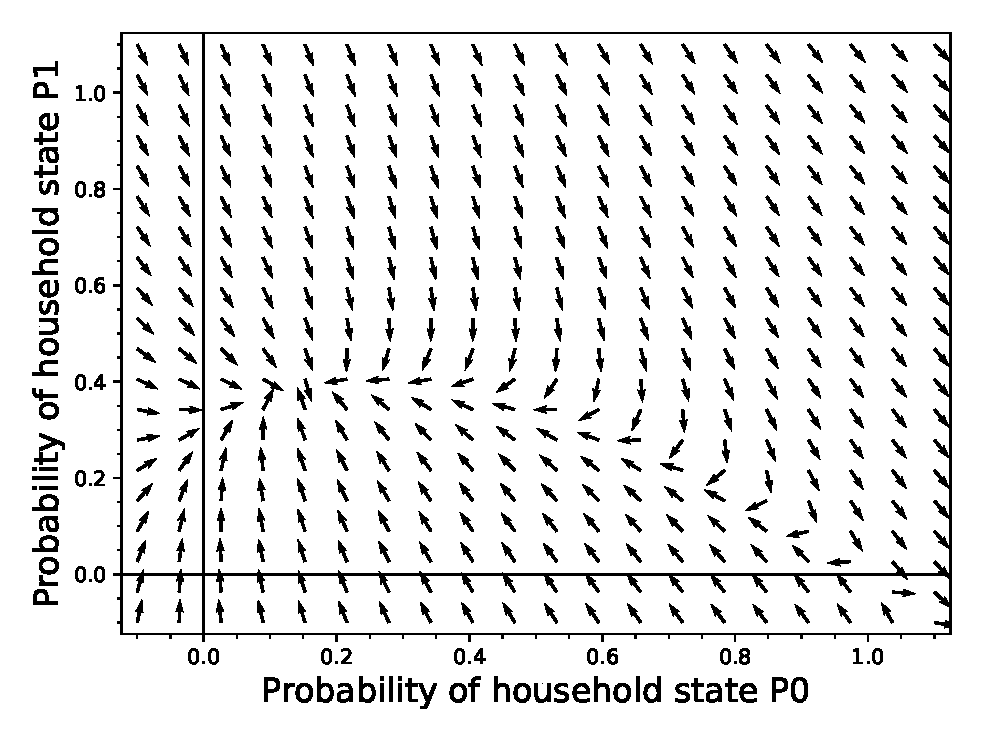
\includegraphics[width=\linewidth]{phase_portrait/01g1.eps}
	   \caption{\(\alpha=0.4, \beta=0.2, \gamma=0.2\)}
	   \label{alpha four phasevectorfield}
	\end{subfigure}
	\begin{subfigure}[b]{0.4\linewidth}
	   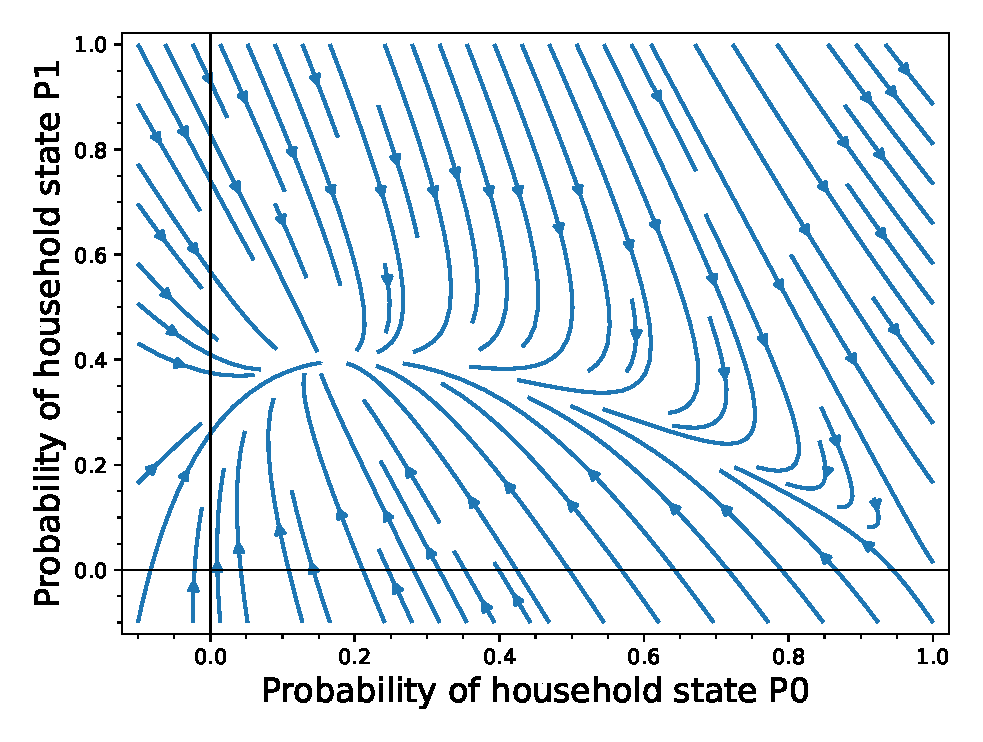
\includegraphics[width=\linewidth]{phase_portrait/01g1s.eps}
	   \caption{\(\alpha=0.4, \beta=0.2, \gamma=0.2\)}
	   \label{alpha four phasestreamplot}
	\end{subfigure}
	\begin{subfigure}[b]{0.4\linewidth}
	  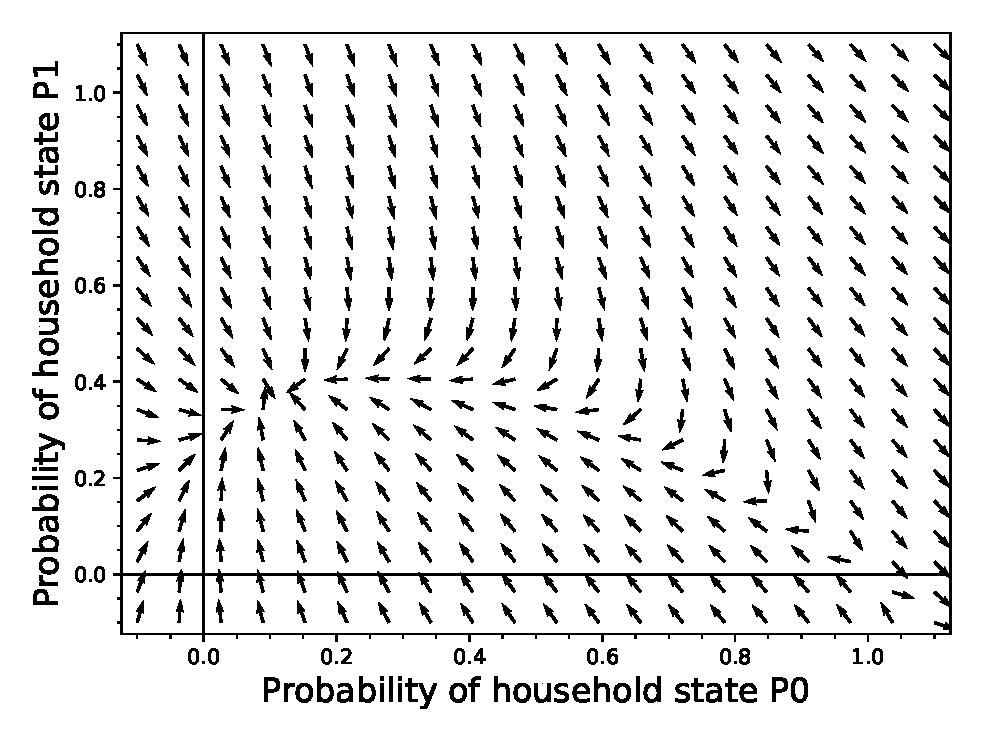
\includegraphics[width=\linewidth]{phase_portrait/021_g2.eps}
	  \caption{\(\alpha=0.5, \beta=0.2, \gamma=0.2\)}
	  \label{alpha five phasevectorfield}
	\end{subfigure}
	\begin{subfigure}[b]{0.4\linewidth}
	  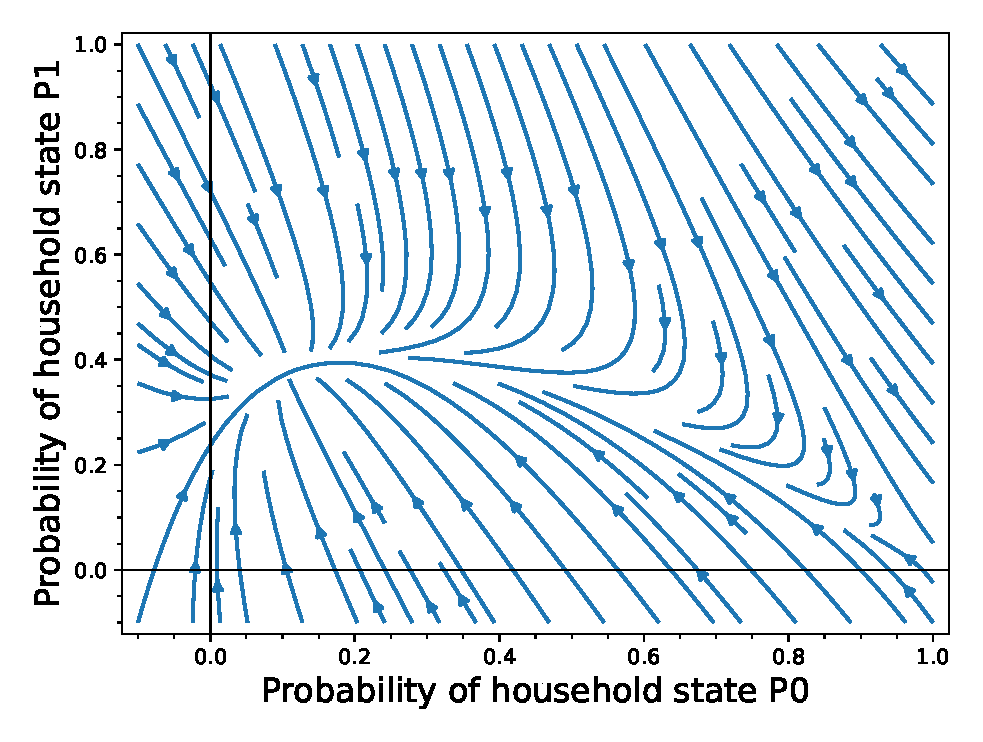
\includegraphics[width=\linewidth]{phase_portrait/021_g2s.eps}
	  \caption{\(\alpha=0.5, \beta=0.2, \gamma=0.2\)}
	  \label{alpha five phasestreamplot}
	\end{subfigure}
	\begin{subfigure}[b]{0.4\linewidth}
	  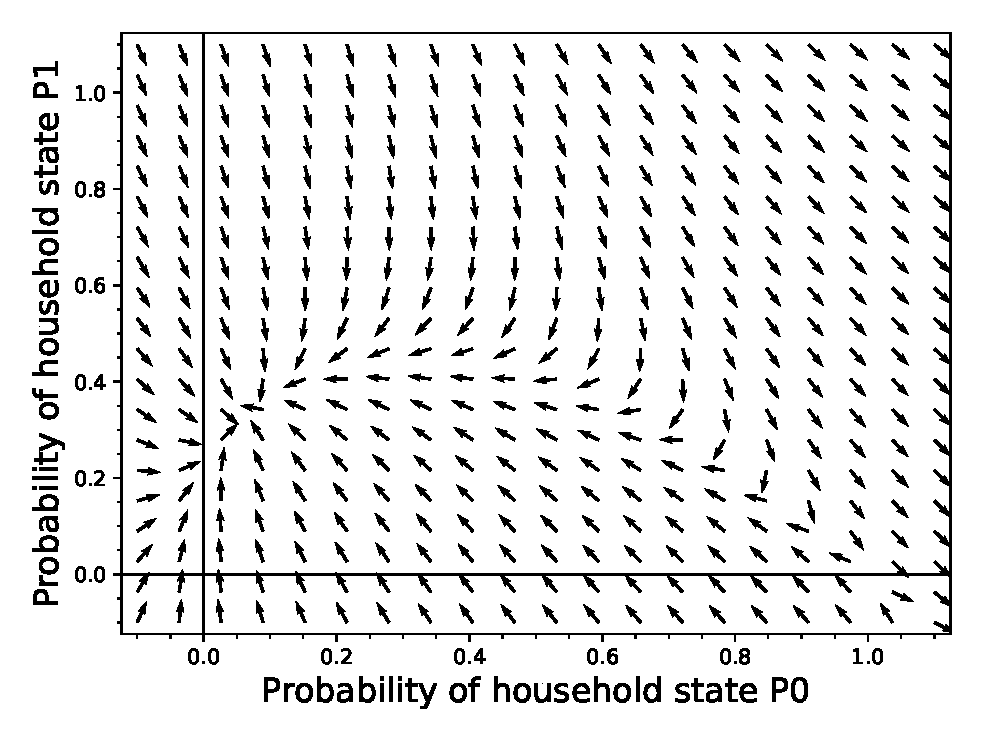
\includegraphics[width=\linewidth]{phase_portrait/031_g4.eps}
	  \caption{\(\alpha=0.7, \beta=0.2, \gamma=0.2\)}
	  \label{alpha seven phasevectorfield}
	\end{subfigure}
    \begin{subfigure}[b]{0.4\linewidth}
	  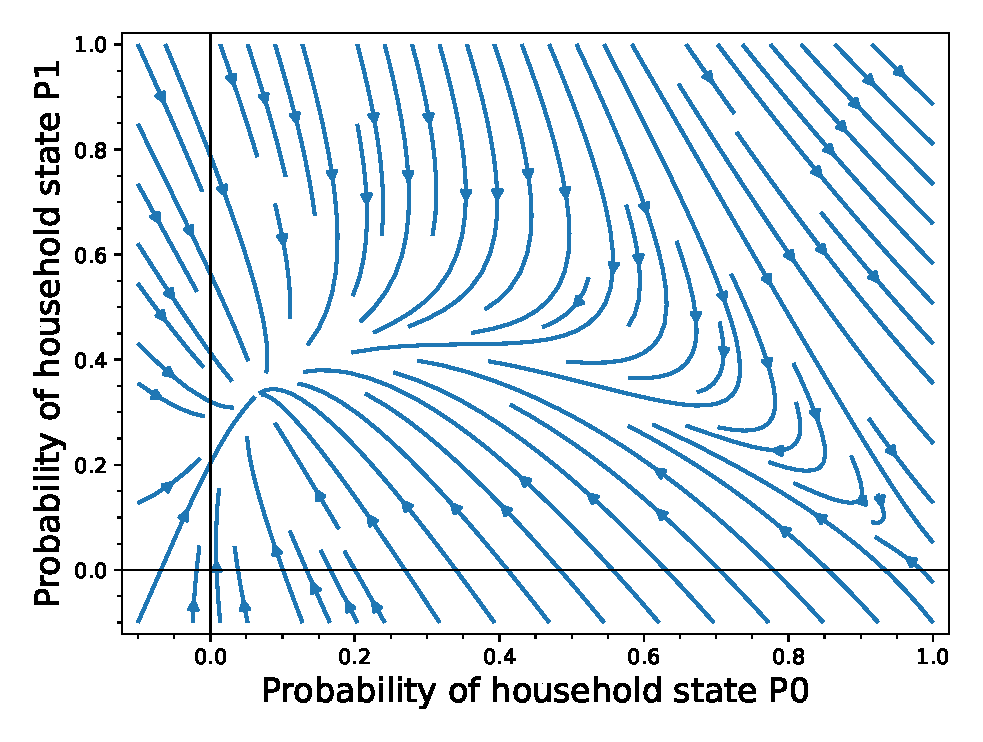
\includegraphics[width=\linewidth]{phase_portrait/031_g4s.eps}
	  \caption{\(\alpha=0.7, \beta=0.2, \gamma=0.2\)}
	  \label{alpha seven phasestreamplot}
	\end{subfigure}
	\begin{subfigure}[b]{0.4\linewidth}
	  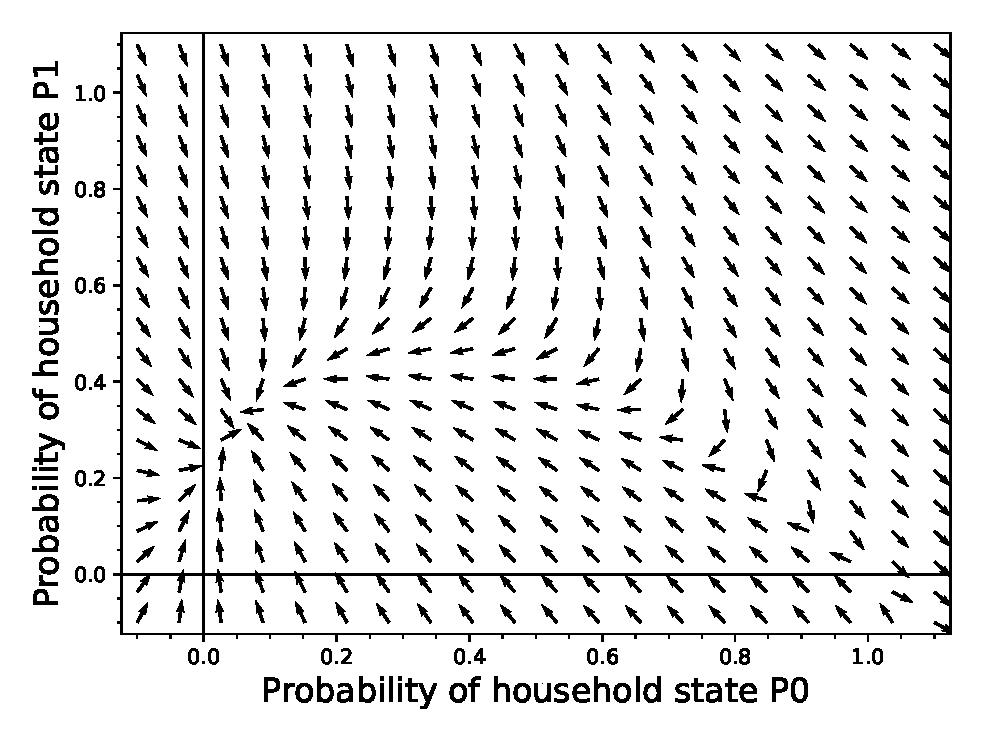
\includegraphics[width=\linewidth]{phase_portrait/041_g5.eps}
	  \caption{\(\alpha=0.8, \beta=0.2, \gamma=0.2\)}
	  \label{alpha eight phasevectorfield}
	\end{subfigure}
	\begin{subfigure}[b]{0.4\linewidth}
	  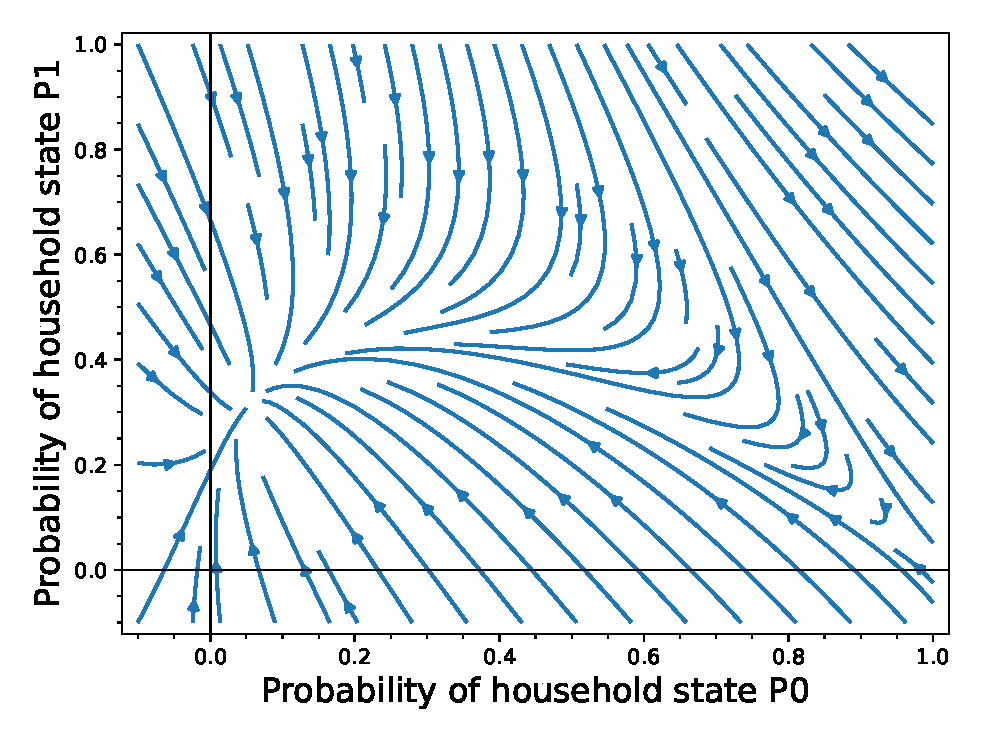
\includegraphics[width=\linewidth]{phase_portrait/041_g5s.eps}
	  \caption{\(\alpha=0.8, \beta=0.2, \gamma=0.2\)}
	  \label{alpha eight phasestreamplot}
	\end{subfigure}
	\caption{Probability of household state P0 = $P_0$ on $x-axis$ and Probability of household state P1 = $P_1$ on $y-axis$ varying $\alpha$.}
	\label{plot of vector fields of $P_0$ on x axis and $P_1$ on y axis of alpha}
\end{figure}
In the above Figure \ref{plot of vector fields of $P_0$ on x axis and $P_1$ on y axis of alpha}, within the \(P_0\) and \(P_1\) plane, we observe two distinct regions at equilibrium. At the equilibrium point (1,0), the disease-free equilibrium acts as a repellor region in the \(P_0\) plane, commonly referred to as a saddle point. The attractor region in both \(P_0\) and \(P_1\) corresponds to the endemic equilibrium. In Figure \ref{plot of vector fields of $P_0$ on x axis and $P_1$ on y axis of alpha}, the gradual increase in \(\alpha\) from 0.4 to 0.8 indicates a sink or attractor region at $P_0$ and $P_1$ plane, which is stable, signifying the existence of an endemic equilibrium. 

\paragraph*{Phase portraits of $P_0$ and $P_1$ with varying $\beta$}\
In this section, we present the phase portrait of \(P_0\) and \(P_1\), varying with \(\beta\) at 0.2, 0.3, 0.4, and 0.5, while keeping \(\alpha = 0.4\) and \(\gamma = 0.2\) fixed in Equation \ref{two dimension}. The visualization includes vector fields and streamline plots.
\begin{figure}[H]
	\centering
	\begin{subfigure}[b]{0.4\linewidth}
	  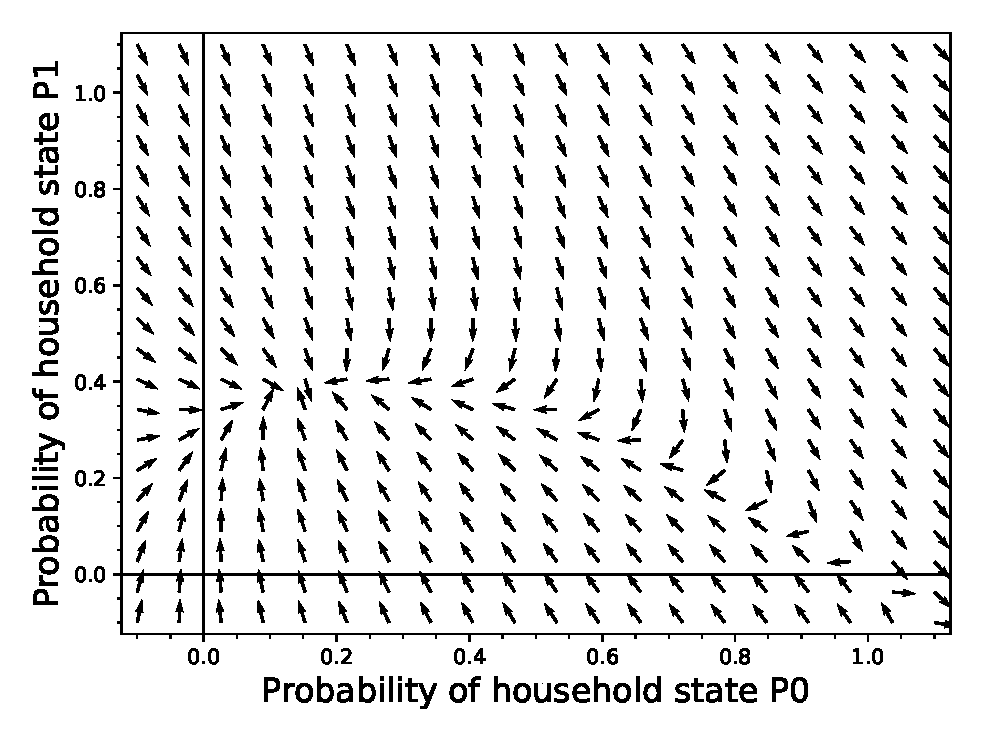
\includegraphics[width=\linewidth]{phase_portrait/01g1.eps}
	  \caption{\(\alpha=0.4, \beta=0.2, \gamma=0.2\)}
	  \label{beta two phasevectorfield}
	\end{subfigure}
    \begin{subfigure}[b]{0.4\linewidth}
	  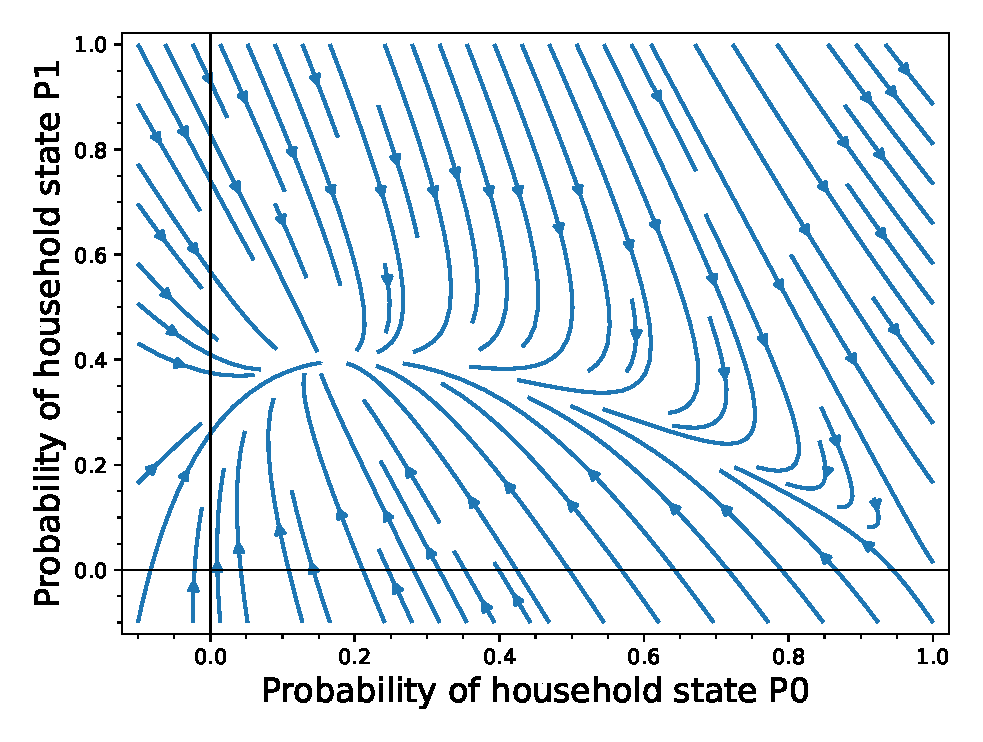
\includegraphics[width=\linewidth]{phase_portrait/01g1s.eps}
	  \caption{\(\alpha=0.4, \beta=0.2, \gamma=0.2\)}
	  \label{beta two phasestreamplot}ex

	\end{subfigure}
	\begin{subfigure}[b]{0.4\linewidth}
	  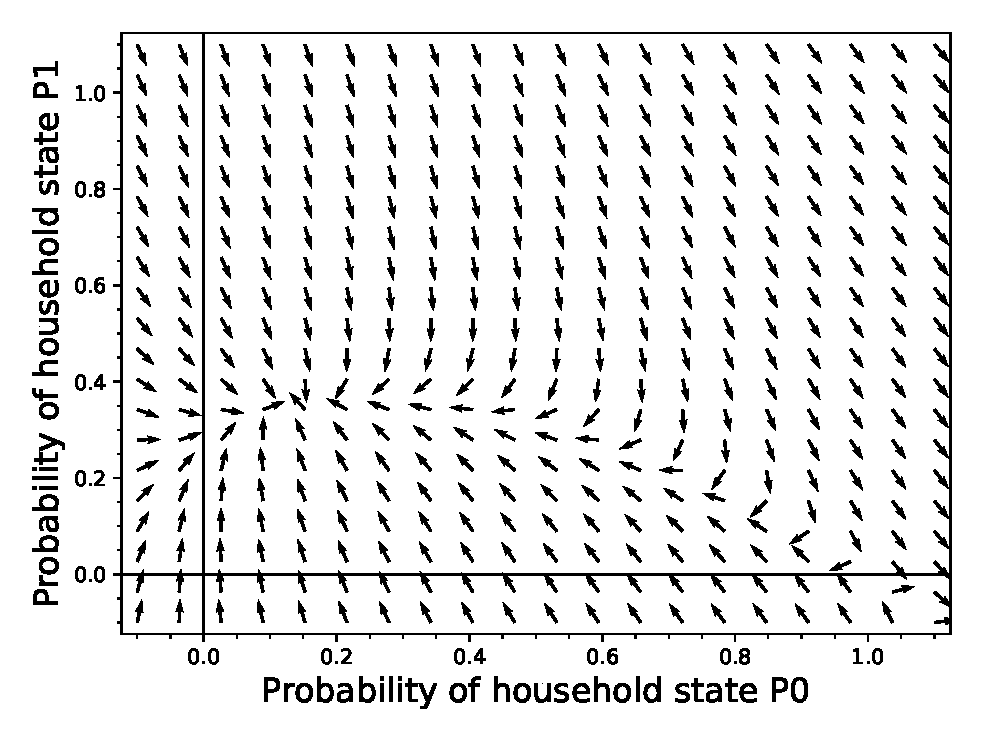
\includegraphics[width=\linewidth]{phase_portrait/022_g6.eps}
	  \caption{\(\alpha=0.4, \beta=0.3, \gamma=0.2\)}
	  \label{beta three phasevectorfield}
	\end{subfigure}
      \begin{subfigure}[b]{0.4\linewidth}
	  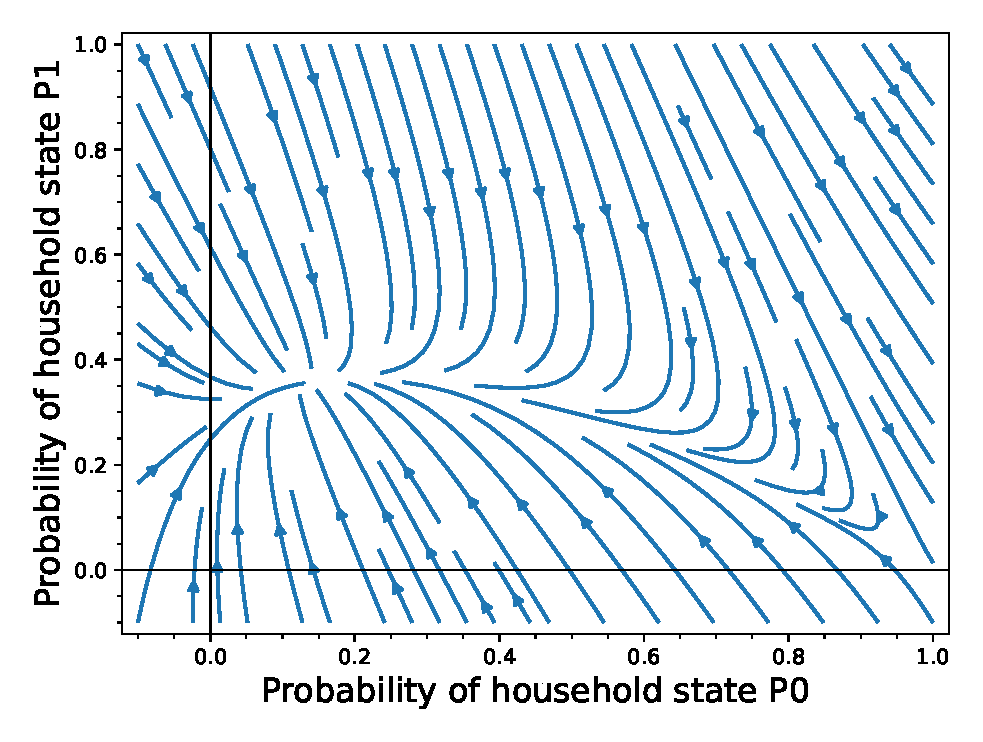
\includegraphics[width=\linewidth]{phase_portrait/022_g6s.eps}
	  \caption{\(\alpha=0.4, \beta=0.3, \gamma=0.2\)}
	  \label{beta three phasestreamplot}
	\end{subfigure}
	\begin{subfigure}[b]{0.4\linewidth}
      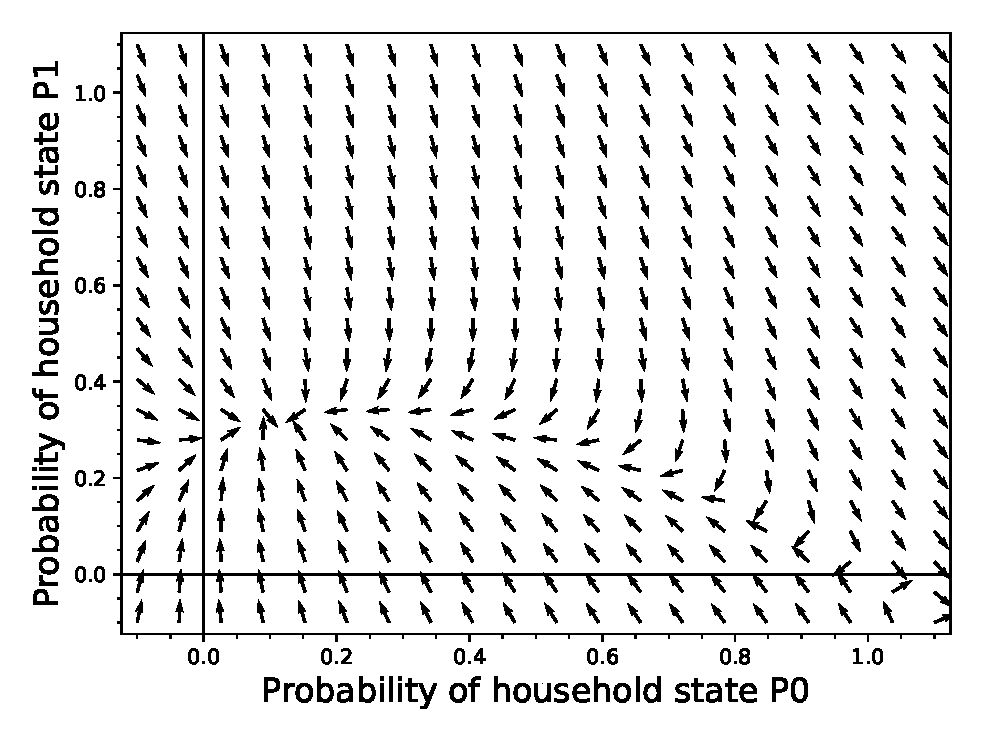
\includegraphics[width=\linewidth]{phase_portrait/032_g11.eps}
	  \caption{\(\alpha=0.4, \beta=0.4, \gamma=0.2\)}
	  \label{beta four phasevectorfield}
	\end{subfigure}
	  \begin{subfigure}[b]{0.4\linewidth}
      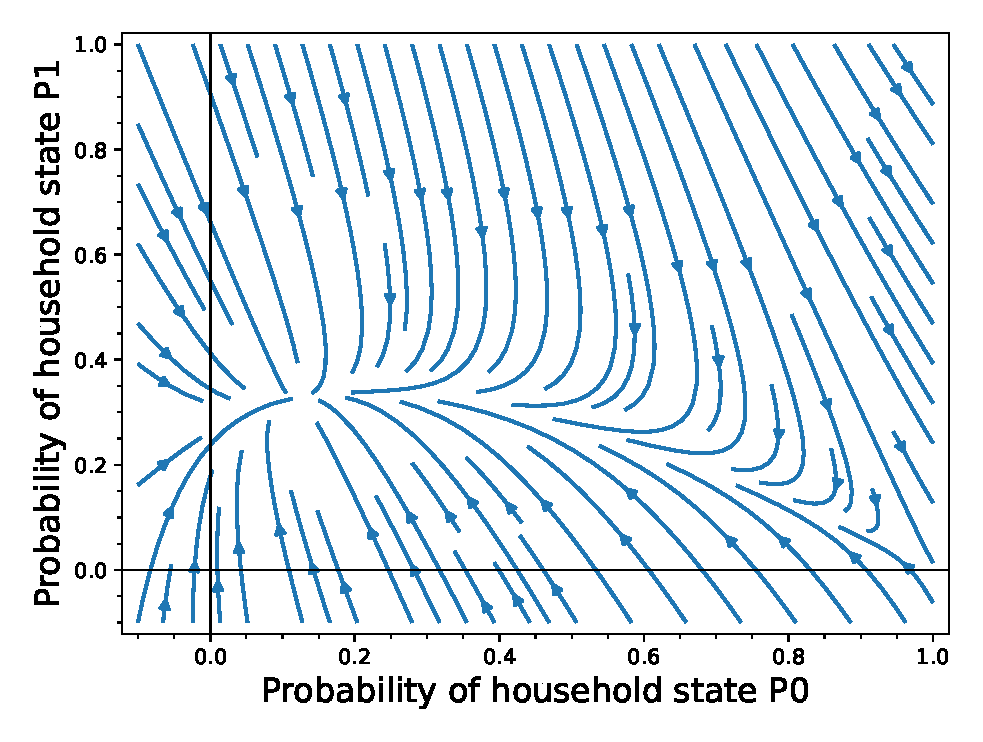
\includegraphics[width=\linewidth]{phase_portrait/032_g11s.eps}
	  \caption{\(\alpha=0.4, \beta=0.4, \gamma=0.2\)}
	  \label{beta four phasestreamplot}
	\end{subfigure}
	\begin{subfigure}[b]{0.4\linewidth}
	  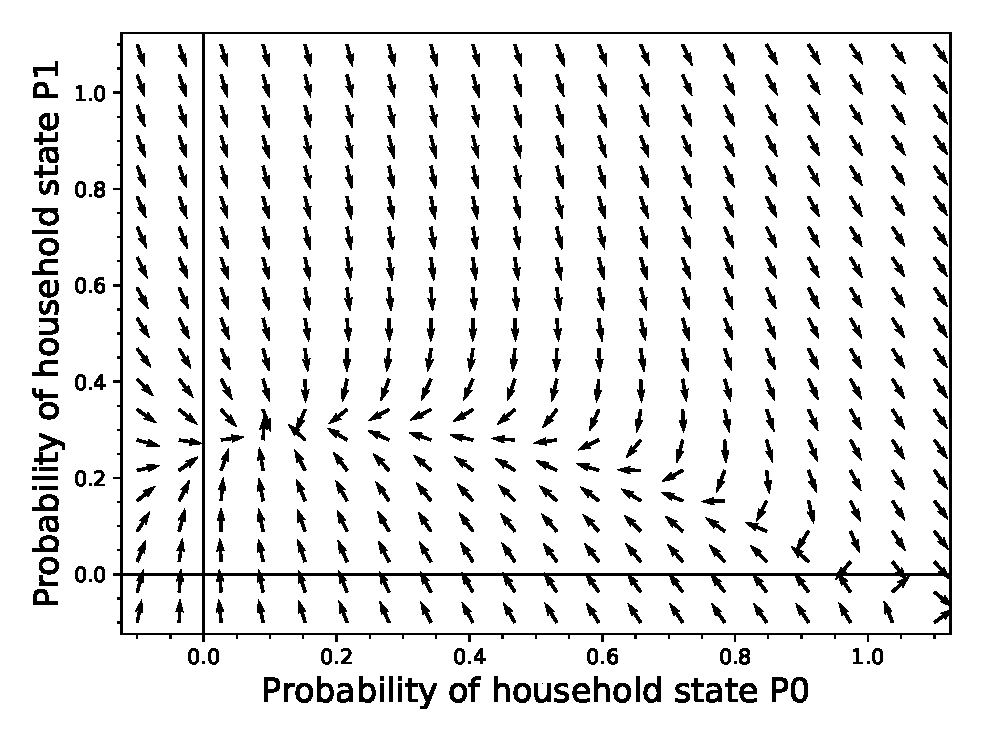
\includegraphics[width=\linewidth]{phase_portrait/042_g16.eps}
	  \caption{\(\alpha=0.4, \beta=0.5, \gamma=0.2\)}
	  \label{beta five phasevectorfield}
	\end{subfigure}
	\begin{subfigure}[b]{0.4\linewidth}
	  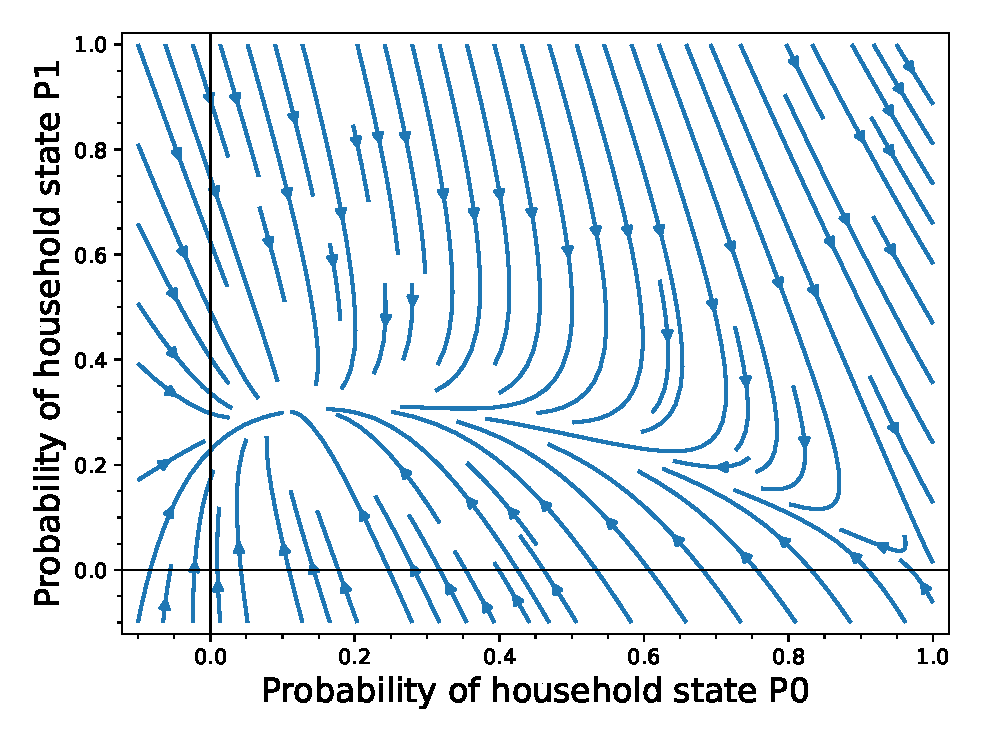
\includegraphics[width=\linewidth]{phase_portrait/042_g16s.eps}
	  \caption{\(\alpha=0.4, \beta=0.5, \gamma=0.2\)}
	  \label{beta five phasestreamplot}
	\end{subfigure}
	\caption{Probability of household state P0 = $P_0$ on $x-axis$ and Probability of household state P1 = $P_1$ on $y-axis$ varying $\beta$.}
	\label{plot of vector fields of $P_0$ on x axis and $P_1$ on y axis for beta}
\end{figure}


In the above Figure \ref{plot of vector fields of $P_0$ on x axis and $P_1$ on y axis for beta}, similar regions are observed when compared to Figure \ref{plot of vector fields of $P_0$ on x axis and $P_1$ on y axis of alpha}. All figures demonstrate stable regions, attractor regions, or sink regions at '\(P_0\) and \(P_1\)' plane , where the disease becomes endemic with a gradual increase in \(\beta\). The region at \(P_0\) (1,0), representing the disease-free equilibrium, shows a repellor or saddle, implying that any introduction of the disease leads to an endemic state.

\paragraph*{Phase portrait of $P_0$ and $P_1$ with varying $\gamma$}\
In this section, we present the phase plane plot with \(\gamma\) varying at rates \(\gamma\) with 0.3, 0.4, 0.6, and 0.8, while keeping \(\alpha = 0.4\) and \(\beta = 0.2\) fixed in Equation \ref{two dimension}. The visualization includes vector fields and streamline plots.
	
\begin{figure}[H]
	\centering
	\begin{subfigure}[b]{0.4\linewidth}
	  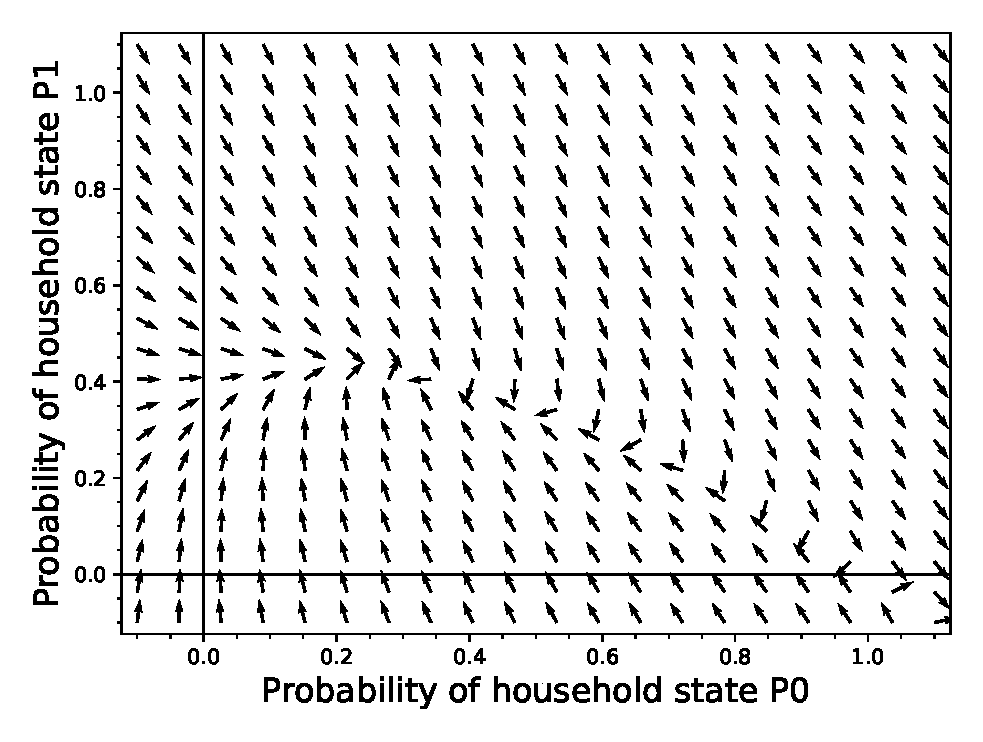
\includegraphics[width=\linewidth]{phase_portrait/023_b6.eps}
	  \caption{\(\alpha=0.4, \beta=0.2, \gamma=0.3\)}
	  \label{gamma three phasevectorfield}
	\end{subfigure}
	\begin{subfigure}[b]{0.4\linewidth}
	  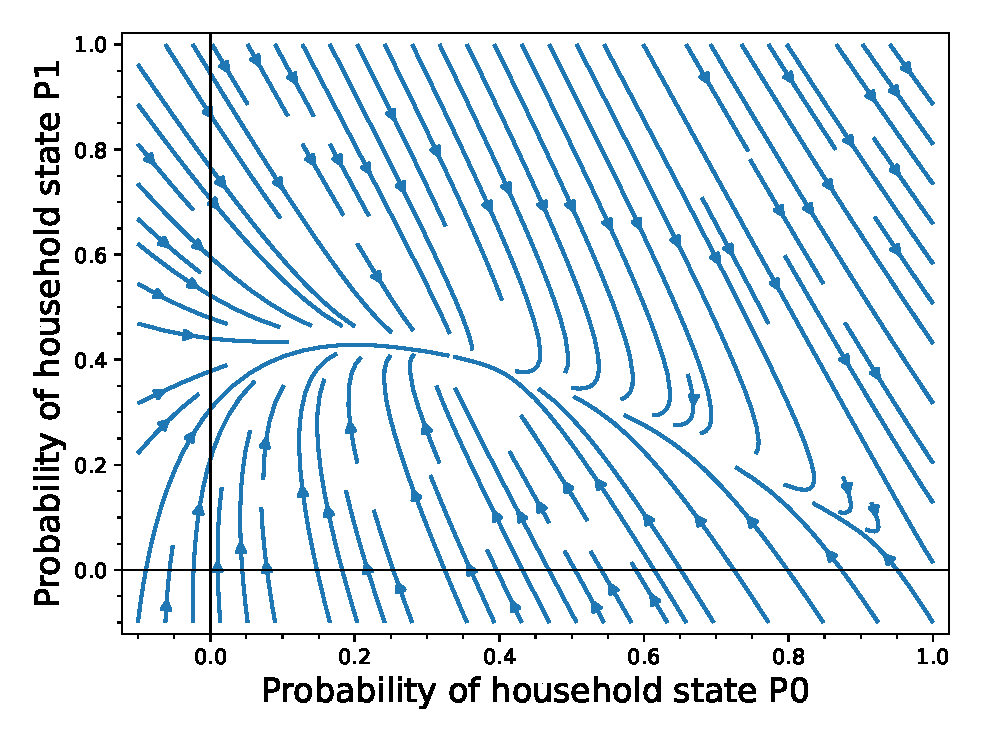
\includegraphics[width=\linewidth]{phase_portrait/023_b6s.eps}
	  \caption{\(\alpha=0.4, \beta=0.2, \gamma=0.3\)}
	  \label{gamma three phasestreamplot}
	\end{subfigure}
    \begin{subfigure}[b]{0.4\linewidth}
	  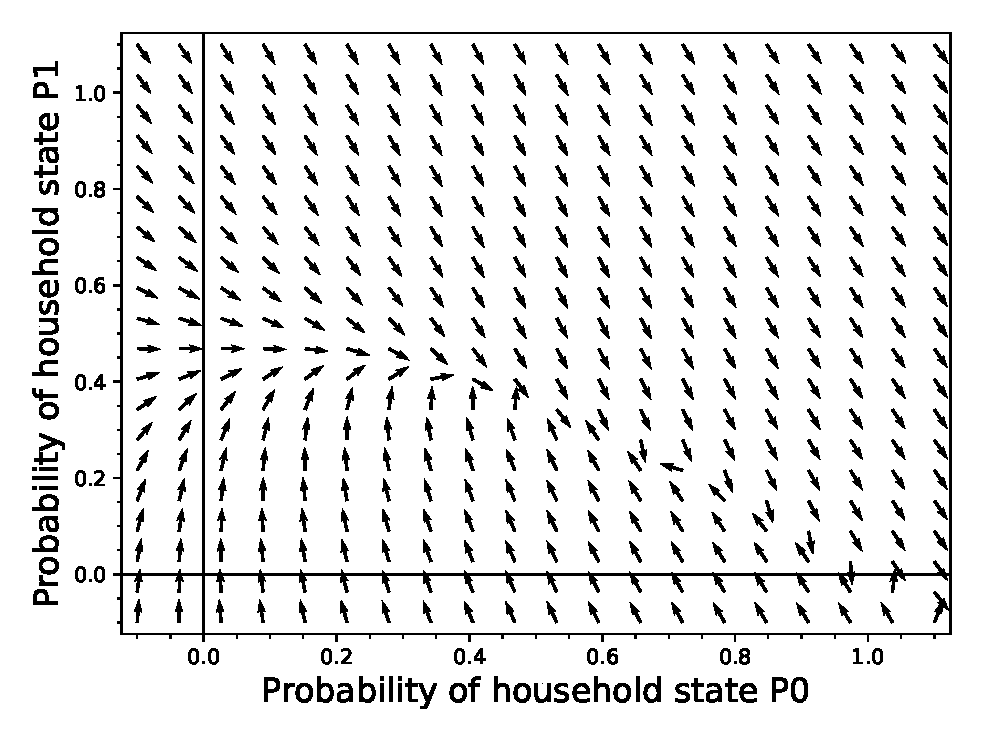
\includegraphics[width=\linewidth]{phase_portrait/033_a1.eps}
	  \caption{\(\alpha=0.4, \beta=0.2, \gamma=0.4\)}
	  \label{gamma four phasevectorfield}
	\end{subfigure}
	\begin{subfigure}[b]{0.4\linewidth}
	  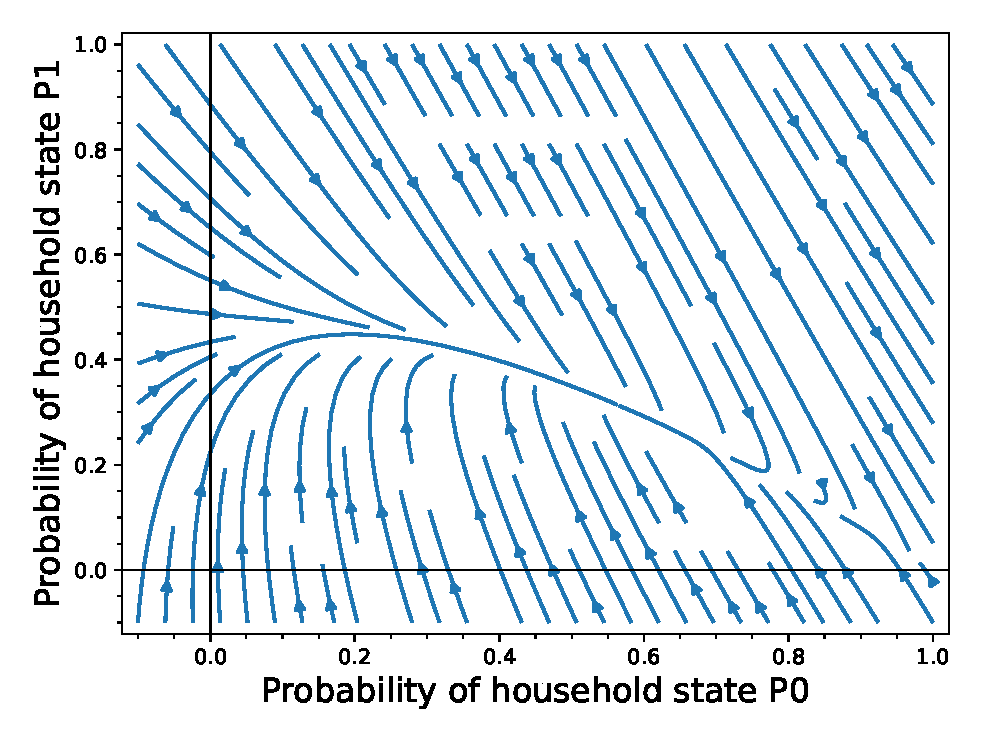
\includegraphics[width=\linewidth]{phase_portrait/033_a1s.eps}
	  \caption{\(\alpha=0.4, \beta=0.2, \gamma=0.4\)}
	  \label{gamma four phasestreamplot}
	\end{subfigure}
	\begin{subfigure}[b]{0.4\linewidth}
		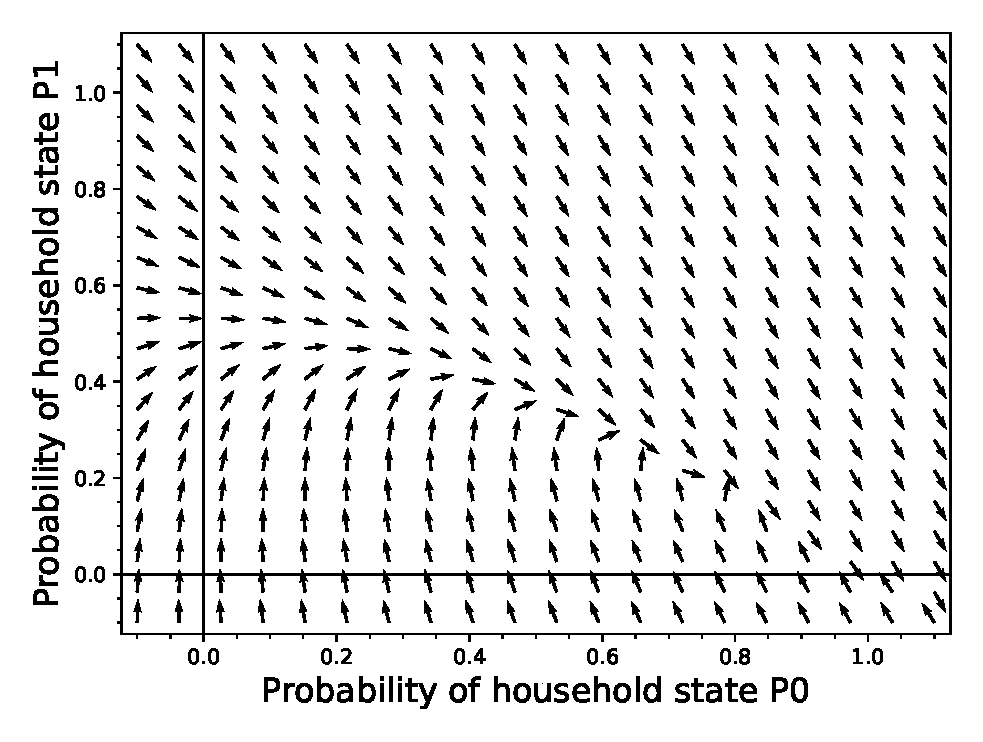
\includegraphics[width=\linewidth]{phase_portrait/043_a3.eps}
		\caption{\(\alpha=0.4, \beta=0.2, \gamma=0.6\)}
		\label{gamma six phasevectorfield}
	\end{subfigure}
	\begin{subfigure}[b]{0.4\linewidth}
		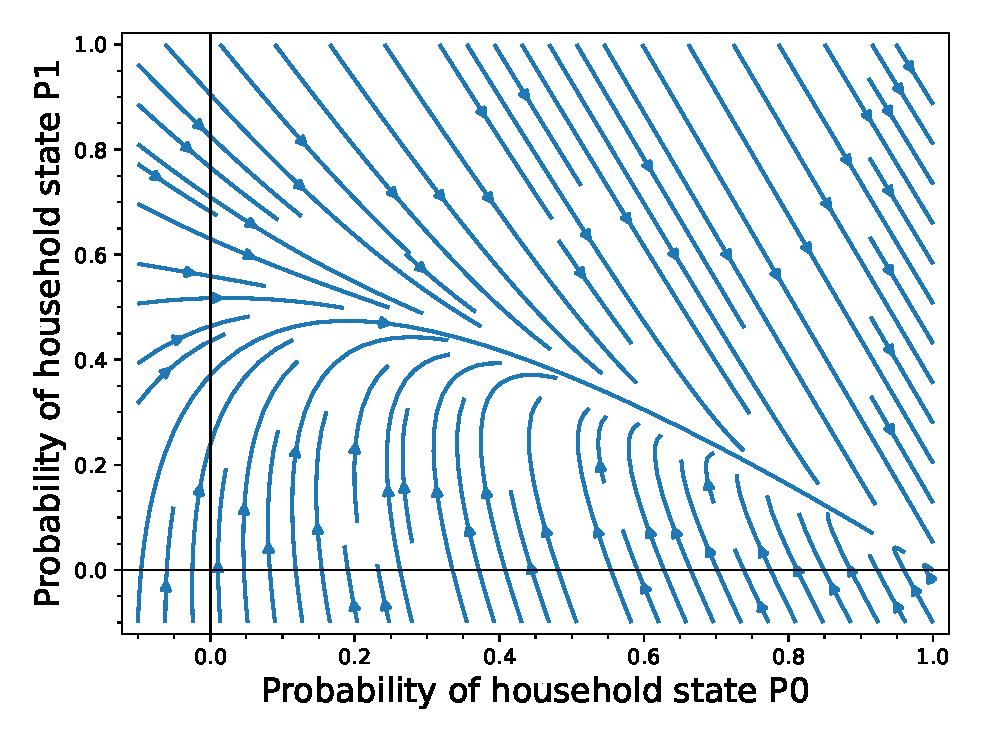
\includegraphics[width=\linewidth]{phase_portrait/043_a3s.eps}
		\caption{\(\alpha=0.4, \beta=0.2, \gamma=0.6\)}
		\label{gamma six phasestreamplot}
	\end{subfigure}
	\begin{subfigure}[b]{0.4\linewidth}
		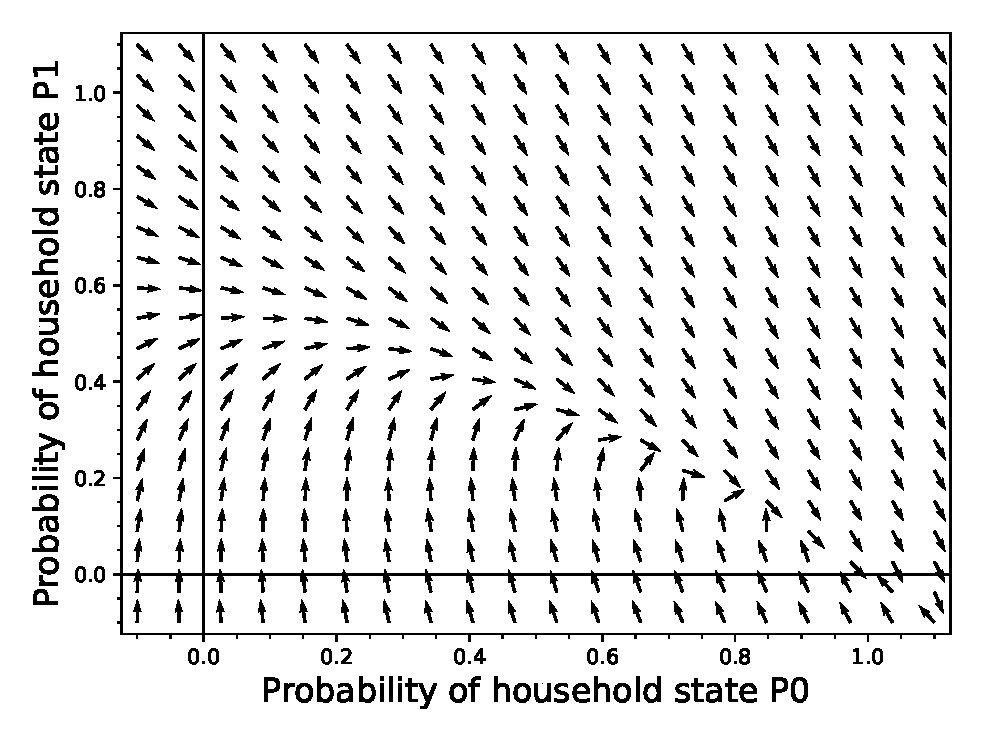
\includegraphics[width=\linewidth]{phase_portrait/043_a5.eps}
		\caption{\(\alpha=0.4, \beta=0.2, \gamma=0.8\)}
		\label{gamma eight phasevectorfield}
	\end{subfigure}
	\begin{subfigure}[b]{0.4\linewidth}
		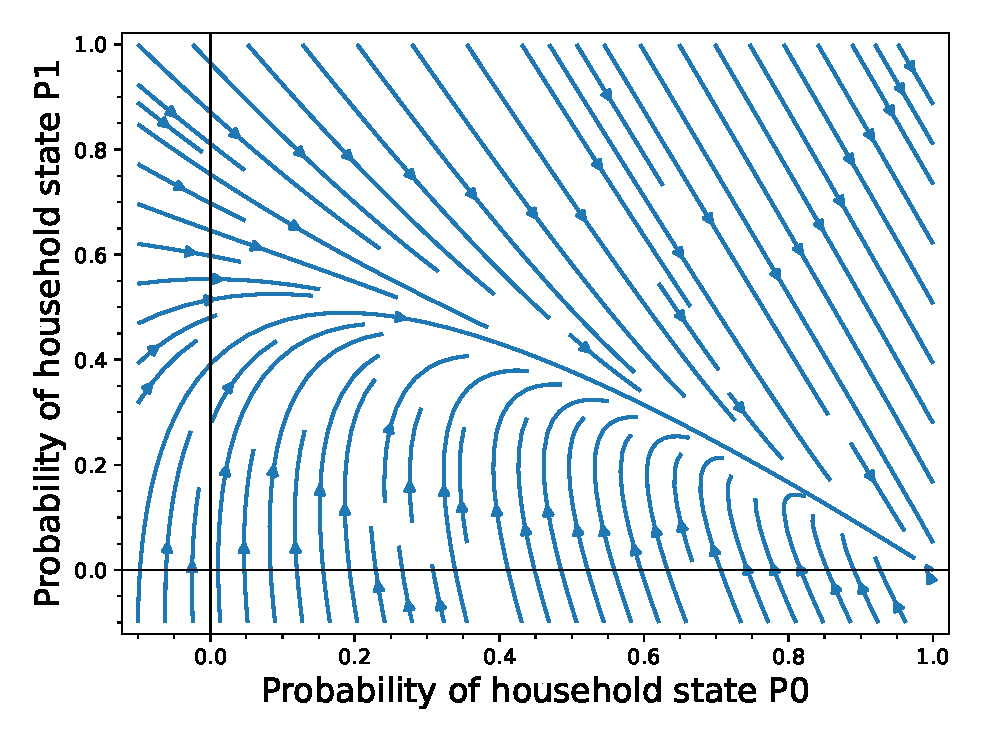
\includegraphics[width=\linewidth]{phase_portrait/043_a5s.eps}
		\caption{\(\alpha=0.4, \beta=0.2, \gamma=0.8\)}
		\label{gamma eight phasestreamplot}
	\end{subfigure}
	\caption{Probability of household state P0 = $P_0$ on $x-axis$ and Probability of household state P1 = $P_1$ on $y-axis$ of $\gamma$.}
	\label{plot of vector fields of $P_0$ on x axis and $P_1$ on y axis for gamma}
   \end{figure}
  %...
In Figures \ref{gamma three phasevectorfield} and \ref{gamma three phasestreamplot}, \(\gamma = 0.3\), and in Figures \ref{gamma four phasevectorfield} and \ref{gamma four phasestreamplot}, \(\gamma = 0.4\), stable regions are observed at plane '\(P_0\) and \(P_1\)' leading disease to endemic, which gradually degenerate at \ref{gamma six phasevectorfield} and \ref{gamma six phasestreamplot}. At \(\gamma = 0.6\) it shows stability at \(P_0\) (1,0) plane leading to disease-free equilibrium.

\chapter{Discussion}

We studied SIS dynamics in a single household of size two. We derived general master equations and applied them to a single household of size two to understand dynamical behaviour of the solutions. 
With numerical simulation performed on master equations, we analyzed parameter by varying between-household infection rate ($\alpha$), within-household infection rate ($\beta$) and recovery rate($\gamma$). We then took on the  epidemiological perspective and assumed a situation where infectious disease enters by introducing 12 infected indiviudals to a small community of 600 households each of size two. Then we studied the disease prevalence with respect to long term and analyze equilibria in disease.\\
%SIS, Homogenousrate SHH, master equation, deterministic,  
\paragraph*{Numerical simulation results discussion}
We performed numerical simulation by using Runge-Kutta method to study master equations in long term behaviour. For simulation, we assumed initial parameters such as between-household infection at a rate of 0.4, within  household infection at 0.2 and recovery rate at 0.2. This initial choice of parameters resulted in lower value in $P_0$ compared to $P_1$ and while comparing $P_1$ to $P_2$, $P_1$ has lower value than $P_2$. 
\subparagraph*{Total Timestep} :

We observed that the gradual increase in the between-household infection rate (\(\alpha\)) leads to a decrease in the total timestep required for all the probability of household states to reach steady states. Similarly, the gradual increase in the between-household infection rate reduces the total timestep needed for the total infection rate and the total recovery rate to reach steady states. In comparison, the gradual increase in the within-household infection rate (\(\beta\)) results in a decrease in the total timestep for all household states to reach steady state. Likewise, the gradual increase in the within-household infection rate decreases the total timestep for the total infection rate and the total recovery rate to reach steady states.\\

When comparing the gradual increase in the within-household infection rate with the between-household infection rate, the total timestep taken by all the probability of household states is less in the between-household infection rate but more in the within-household infection rates. Similarly, when comparing the within-household infection rate with the between-household infection rate, the total timestep taken by the total infection rate and the total recovery rate is more in the within-household infection rate but less in the between-household infection rate. \\
Meanwhile, the total timestep taken by all the probabilities of household states, considering both the total infection rate and the total recovery rate, increases gradually with the rise in the recovery rate until reaching steady states, up to a rate of 0.5.  
\subparagraph*{Changes in the total values of a probability of household state, total infection rate and total recovered rate with parameters $\alpha$, $\beta$ and $\gamma$}:
The gradual increase in the between-household infection rate from 0.4 to 0.8 further decreases the values of \(P_0\) and \(P_1\) but increases the value of \(P_2\), as illustrated in Figure \ref{discrete alpha values}.

Similarly, we observed that the gradual increase from 0.3 to 0.5 in the within-household infection rate decreases the values of \(P_0\) and \(P_1\) but increases the value of \(P_2\), as shown in Figure \ref{discrete beta values}.

Comparing the changes between the within-household and the between-household infection rates in all the probability of household states, \(P_0\) decreases more with the gradual increase in the between-household infection rate but decreases less with the gradual increase in the within-household infection rate. Conversely, for \(P_1\), it decreases less with the between-household infection rate but more with the within-household infection rate, as seen in Table \ref{tab Probability of Household state values varying alpha} and \ref{table Household state values varying beta}. The value of \(P_2\) remains similar with the gradual increase in both between-household and within-household infection rates. In the case of the total infection rate and the total recovery rate, both increase with the gradual increase in both between-household and within-household infection rates, but the gradual increase in the between-household infection is more than in the within-household infection rate.

Regarding the household recovery rate, a gradual increase from 0.3 to 0.6 resulted in a high increase in \(P_0\) but a sharp decrease in both \(P_1\) and \(P_2\), as shown in Figure \ref{discrete gamma values }. The total infected rate and total recovery rate decrease with a gradual increase in the recovery rate. At the recovery rate \(\gamma = 0.6\), \(P_1\) and \(P_2\) become negligible to zero.

\paragraph*{Endemic Equilibrium(EE)}:
We interpreted the values for $P_0$, $P_1$ and $P_2$ in our results section with the equations at \ref{positive root of P0}, \ref{positive root of P1} and \ref{positive root P2}. 
We used linearization near equilibrium points. And the Jacobian at equilibirum solutions to calculate eigenvalues. Among the three calculated eigenvalues, two negative eigenvalues confirm stability around the equilibrium solution. The other zero eigenvalue did not provide any qualitative analysis. We found that the calculated negative eigenvalues decrease with the gradual increase in the between-household infection rate. Similarly, we also found that the calculated negative eigenvalues decrease with the gradual increase in the within-household infection rate. Likewise, in the recovery rate, we also observed a decrease in the negative eigenvalues till recovery rate at 0.5. 

\paragraph*{Disease-Free Equilibrium(DFE)}
After the gradual increase in the recovery rate, $P_1$ and $P_2$ became negligible to zero, and at $\gamma=0.6$, stable regions occured at $P_0$ (1,0,0).
We computed the Jacobian at $(1,0,0)$ and found that eigenvalues depend on parameters $\alpha$, $\beta$, and $\gamma$ (see Figure \ref{submatrix}). A case of $Tr < 0$ and $Tr > \sqrt{Tr^2-4D}$, where $D > 0$, $Tr^2 > 4D$, was crucial in finding negative eigenvalues as regions for stability. In this case, when $Tr < 0$, the $\alpha$ rate is strictly less than $\beta$ and $3\gamma$. This can be interpreted as the difference in the between-household infection rate and the within- household infection rate being smaller than compared to the recovery rate. Similarly, the lower rate of $\beta$ and higher rate of $\gamma$ in the of the expression $\alpha < \frac{\gamma^2}{\beta + \gamma}$ of $D > 0$ decides the stable region for the disease-free equilibrium. For a stable region to occur, the recovery rates should be high. Figure \ref{regions of stability and unstability} shows that stable and unstable regions exist in $\gamma$ vs $\beta$ where $\alpha$ is fixed at 0.4. We interpret this scenario as when $\alpha$ is constant and $\beta$ is lower compared to a higher recovery rate, the disease-free equilibrium occurs.

\paragraph*{Phase portrait}:

The influence of varying $\alpha$, $\beta$, and $\gamma$ in the '$P_0$ and $P_1$' plane was also shown by the phase portrait. We observed the endemic equilibrium (EE) and disease-free equilibrium (DFE) at the domain of $P_0$ [0,1] and $P_1$ [0,1]. The gradual increase in $\alpha$ showed stable regions at endemic equilibrium solutions, forming attractor regions or sink regions. Similarly, the gradual increase in $\beta$ showed stable regions at endemic equilibrium solutions but unstable regions at the fixed point (1,0) in the $P_0$ axis, which indicates a repellor or saddle. However, the gradual increase in the recovery rate shifted the stable regions from the $P_0$ and $P_1$ plane towards the fixed point (1,0). At the recovery rate $\gamma=0.6$, the fixed point (1,0) showed stability regions, which have an attractor or sink region, referred to as disease-free equilibrium, as observed in the phase portrait section.

\paragraph*{Limitations}:
At initial stage, we wanted to study about infectious disease in mixed household size rather than same household size but due to limited time, we analyzed equilibria in disease-free equilibrium and endemic equilibrium in a single household of size two. In a household, isolation policy is hard to implement, where everybody in a family interacts with one another. In SHH of size two it is obvious that inside household there is only one individual who is infective and transmit infection to the other susceptible but question arises what would happen with household of larger size where the chances are high that more individuals will be infected. Also the focus was not on crafting strategies or policies based on the results of simulation rather the focus was on analyzing equilbria. Lastly, we did not define the household structure and behavioural patterns of individuals.\\
  

\paragraph*{Further research}
Further reseach on equilibrium can be done on higher dimensions having more than two individuals in a household, which leads to even more complexity in the dynamics. A numerical approximation method like Runge-Kutta could be used to see overall scenario of disease in long term. It would be interesting to observe these scenario in large population and also in a small community.\\  

Further research can be done on other epidemiological models of SIS varitaions SI, SIR, SEIR or other variation according to various form of diseases. Also finding modeling method for policies such vaccination, isolation, herd immunity etc would be beneficial in future for intervention strategies when disease outbreaks. We used linearization method for single household of size two in SIS, further research could be possible in calculating reproduction number and new generation matrix with spectral radius. Also, we studied with high rate of parameters but the study can also be done with low value of parameters to see significant changes in equilibrium.  

\chapter{Conclusion}

In the thesis, we analyzed SIS dynamics in master equations for single household of size two to understand the dynamic behaviour of solutions at an equilibrium condition from the perspective of mathematical epidemiology. 
We considered the course of an infectious disease to be deterministic and homogenous. Then we derived general master equation to understand phenomenon for finite household size. Due to time limitation, we restricted our discussion to analyzing equilibria of disease in a single household of size two. In master equation, we graudally increased the rate between-household infection rate($\alpha$), within-household infection rate($\beta$) and recovery rate($\gamma$)'s and investigated the influence on a single household of size two. Our SHH approximation in SIS model showed both endemic equilibrium and disease-free equilibrium and confirmed it by analytical finding. We observed that $P_0$ and $P_1$ decreases with graudal increase in between-household infection rate and within-household infection rate. On the other hand $P_2$ and total infection rate increases with gradual increase in between-household infection rate and within-household infection rate. Moreover $P_1$, $P_2$ and total infection rate decreases with gradual increase in recovery rate. Conversely $P_0$ increases with gradual increase in recovery rate. \\
In summary, a transition from endemic equilibrium to a disease-free equilibrium is observed when the recovery rate is set at 0.6. This transition occurs within a specific range of household transmission rates, particularly when the between-household rate is set at 0.4 and the within-household rate is at 0.2.  

%%%
%%% If there is some appendix, remove the comments
%%% Otherwise comment it out or delete it
%\appendix
%\chapter{An appendix chapter}

%% Biblipgraphy
%% using bibtex, bibtex-File mybiblio.bib
%% For compilation: 2x LaTeX, 1xbibTeX, 2xLaTeX

\bibliographystyle{plain}
\bibliography{references}
\end{document}

